\documentclass[12pt,letterpaper]{article}
\usepackage{amsmath, amssymb, amsthm}
\newtheorem{theorem}{Proposition}
\theoremstyle{remark}
\newtheorem*{remark}{Remark}
\usepackage{graphicx}
\usepackage{setspace}
\usepackage{amsmath, amssymb, amsthm}
%\newtheorem{theorem}{Proposition}
\theoremstyle{remark}
%\newtheorem*{remark}{Remark}
\usepackage[T1]{fontenc}
\usepackage{setspace}
\usepackage{pdflscape}
\usepackage{booktabs, threeparttable, tabularx, makecell, siunitx}
\DeclareMathOperator*{\rint}{\ThisStyle{\rotatebox{15}{$\SavedStyle\!\int\!$}}}
\usepackage{indentfirst}
\usepackage{xurl}
\usepackage{threeparttable}
\usepackage{caption}
\usepackage{subcaption}
\usepackage[colorlinks=true,linkcolor=black,urlcolor=blue,citecolor=black]{hyperref}
\usepackage{float}
\newcommand{\floatfoot}[1]{\par\vspace{2pt}\noindent#1}
\makeatletter
\let\oldtable\table
\let\endoldtable\endtable
\renewenvironment{table}[1][H]{\oldtable[H]}{\endoldtable}
\makeatother
\usepackage{pgfplots}
\usepackage[affil-it]{authblk}
\pgfplotsset{compat=1.16}
\usepackage{dcolumn}
\usepackage[osf]{mathpazo}
\usepackage{afterpage}
\usepackage[makeroom]{cancel}
\usepackage{listings}
\usepackage{lscape}
\usepackage[left=2cm,right=2cm,top=1.5cm,bottom=1.5cm]{geometry}
\usepackage{enumitem}
\BeforeBeginEnvironment{tabular}{\footnotesize}% Adjust tabular font size to \small
\usepackage{authblk}
% siunitx setup
\sisetup{table-number-alignment=center, table-figures-integer=2, table-figures-decimal=1}
% Theorem, Lemma, etc
\theoremstyle{plain}
%\newtheorem{theorem}{Theorem}
\newtheorem{corollary}[theorem]{Corollary}
\newtheorem{lemma}[theorem]{Lemma}
\newtheorem{claim}{Claim}[theorem]
\newtheorem{axiom}[theorem]{Axiom}
\newtheorem{conjecture}[theorem]{Conjecture}
\newtheorem{fact}[theorem]{Fact}
\newtheorem{hypothesis}[theorem]{Hypothesis}
\newtheorem{assumption}[theorem]{Assumption}
\newtheorem{proposition}[theorem]{Proposition}
\newtheorem{criterion}[theorem]{Criterion}
\theoremstyle{definition}
\newtheorem{definition}[theorem]{Definition}
\newtheorem{example}[theorem]{Example}
\newtheorem{problem}[theorem]{Problem}
\newtheorem{principle}[theorem]{Principle}

\usepackage{graphicx, color}
\usepackage{booktabs}
\graphicspath{{fig/}}

\usepackage[round,sort,comma,authoryear]{natbib}
\bibliographystyle{apalike}
\bibpunct{(}{)}{,}{a}{,}{,}


%\usepackage[linesnumbered,ruled,vlined,commentsnumbered]{algorithm2e} % use algorithm2e for typesetting algorithms
\usepackage{algorithm, algpseudocode} % use algorithm and algorithmicx for typesetting algorithms
\usepackage{mathrsfs} % for \mathscr command


\title{Crop Sequence Timing, Corn Yields, and Yield Risk: A Just-Pope Analysis}

\author[1]{Victor Funes-Leal}
\author[2]{Lawson Connor}
\author[3]{Eunchun Park}
\affil[1,2,3]{Department of Agricultural Economics and Agribusiness, University of Arkansas}
\date{}

\begin{document}

\maketitle
\begin{abstract}
\noindent
We investigate how the timing and spacing of soybean placement within long-term crop rotation sequences affect corn yields, using a large, satellite-based, field-level panel of Illinois corn yields for 2008 to 2022, with rotation histories built from Cropland Data Layer records back to 2002. We pair field-level corn yield estimates from the Quantile Loss Domain Adversarial Neural Networks estimator (QDANN) with six-year crop-sequence histories from the USDA Cropland Data Layer, and estimate linear fixed-effects models that separately identify sequence effects on the conditional mean and variance of yields, following \citet{Just1979}. Rotation effects depend on the timing and spacing of soybean placements: a recent soybean harvest and a wider gap between soybean years each raise mean corn yields, and the highest-performing sequences carry premiums of roughly four to six bushels per acre over continuous corn. A LASSO-based sequence selection exercise recovers the same recency pattern from the data alone, without an assumed functional form. The effects on yield risk are less precisely estimated but share the direction of the mean effects: wider soybean spacing is associated with lower yield variance, significant under the pairs cluster bootstrap used for the variance stage though only marginal under analytic standard errors. Effects on the third moment of the yield distribution run the other way: the sequences with a detectable skewness effect shift probability mass toward the left tail relative to monoculture, so few if any sequences achieve full three-moment dominance over continuous corn. We summarize the structural features driving the mean and variance results in a single rotation score that maps the observed six-year sequences onto a scalar rating scale spanning approximately $-2.68$ to $+1.88$ relative to corn monoculture. These results are directly relevant to proposals for rotation-conditioned federal crop insurance rates; a companion paper examines whether the Rotational Complexity Index (RCI), the standard scalar summary of rotation diversity, and spatial spillovers across neighboring fields, carry the same information.

\medskip\noindent
\textbf{Keywords:} crop rotation, crop insurance, Just-Pope production risk, yield variance, sequence timing, Illinois, satellite yields.

\medskip\noindent
\textbf{JEL Codes:} Q12, Q18, G22, C23.
\end{abstract}

\newpage
\setcounter{page}{1}

\section{\label{sec:intro}Introduction}

Crop rotations are among the most widely studied agronomic practices in temperate agriculture, yet their role in federal crop insurance ratings remains largely unexplored. The United States Federal Crop Insurance Program (FCIP) covers more than 90 percent of planted corn and soybean acres in the Midwest, with annual indemnities exceeding \$19 billion in recent years. Premium rates are calculated based on each farm's Actual Production History (APH), a rolling 10-year average yield that forms the actuarial basis for coverage. This design is intentionally farm-specific but blind to the practices that generate the underlying yield record. A farmer who maintains a disciplined corn-soybean rotation, a practice well documented to raise mean yields and reduce yield variability, pays the same actuarially implied premium as a neighboring farmer in continuous corn, conditional on the same APH. This paper asks whether this constitutes a pricing inefficiency and how large the underlying yield differential is, and, if so, what feature of the rotation history actually drives it.

We study how long-term crop rotation sequences affect the mean and variance of corn yields using a large, satellite-based, field-level panel of Illinois corn yields for 2008 to 2022, with rotation histories drawn from Cropland Data Layer records back to 2002. Using field-level corn yield estimates from the Quantile Loss Domain Adversarial Neural Networks estimator \citep[QDANN;][]{Ma2024}, together with field-level crop sequence histories from the USDA Cropland Data Layer (CDL), we estimate linear fixed effects models that separately identify rotation effects on the conditional mean and conditional variance of yields, following \citet{Just1979}. Field and year fixed effects absorb time-invariant field characteristics and common annual shocks, so that identification comes from within-field variation in rotation sequences over time.

Our main findings are three. First, a handful of rotation sequences significantly outperform corn monoculture in mean yields, and these sequences share identifiable structural features -- specifically, a soybean harvest within the past one to two years and adequate spacing between soybean years in the six-year window -- rather than the overall diversity of the rotation. Second, a data-driven LASSO selection over the full candidate sequence space recovers the same recency-and-spacing pattern without imposing it, cross-validating the parametric result. Third, we construct a rotation score from these structural features that maps the observed six-year rotation sequences, drawn from corn, soybean, and winter-wheat histories, onto a scalar index. The score ranges from approximately $-2.68$ to $+1.88$ relative to corn monoculture, normalized to zero, across 28 sequences spanning 14 distinct score values (mean $0.16$, median $0.56$); the perfect alternating rotation (S-C-S-C-S-C) scores $+0.49$.

These findings speak directly to two active policy debates. First, USDA's Risk Management Agency (RMA) has signaled interest in incorporating conservation practice information into crop insurance rating as part of broader efforts to align the FCIP with climate and conservation goals. Our results suggest that rotation history is an actuarially meaningful predictor of yield risk, but incorporating it requires sequence-level or structural-feature-based characterization rather than a simple index; a companion paper shows that the standard scalar alternative, the Rotational Complexity Index (RCI), does not carry this information cleanly. Second, the literature on conservation practice adoption has noted that the APH mechanism may inadvertently discourage rotations and cover cropping by recording short-run yield dips during practice transitions \citep{Connor2022}. Our estimated transition effects provide direct evidence on the magnitude and persistence of this penalty for corn-soybean rotation sequences in Illinois, and our rotation score provides a tractable rating instrument that could condition premiums on rotation history.

The paper proceeds as follows. Section~\ref{sec:litreview} reviews the relevant literature on rotation effects and crop insurance rating. Section~\ref{sec:data} describes our data sources and the construction of rotation sequences. Section~\ref{sec:econ_framework} presents the econometric framework. Section~\ref{sec:results} reports results. Section~\ref{sec:conclusions} discusses implications for insurance rating and concludes.

\section{\label{sec:litreview}Literature Review}
\subsection{\label{subsec:agronomy}Agronomic and Economic Evidence on Crop Rotations}

The agronomic literature has extensively documented the yield benefits of crop rotation. In controlled experimental settings, the corn yield advantage from a preceding soybean year has been estimated at 5 to 15 percent relative to continuous
corn, depending on soil type, nitrogen fertilization rate, and weather conditions \citep{Gentry2013, Farmaha2016}. The primary mechanisms include improved nitrogen availability from soybean residue-particularly net soil nitrogen mineralization that reduces the nitrogen demand of subsequent corn-reduced pathogen and pest pressure, and differences in residue decomposition that affect soil temperature and structure at planting \citep{Gentry2013}.

Observational literature using field- or farm-level data is thinner because isolating the causal effect of rotation from selection on land quality and farmer ability requires either experimental variation or credible panel designs. \citet{burchfield2024} use county-level data across the US Midwest and find that rotational complexity as measured by the RCI is insufficient to generate detectable yield gains at the county scale, a result they attribute to the coarseness of county aggregation and the dominance of the corn-soybean binary in most counties. \citet{socolar2021} find that biophysical and policy factors together predict simplified rotations, with proximity to ethanol infrastructure among the key predictors of monoculture adoption-a finding consistent with the spatial patterns documented by \citet{pates2021} using remote sensing data. Our paper contributes a field-level panel for Illinois that sidesteps the aggregation problem and identifies yield effects within counties across fields over time, focusing on the sequence-level structure of the rotation rather than a scalar diversity summary; a companion paper takes up the scalar-index and spatial-spillover questions directly.

The determinants of rotation choice are themselves the subject of a growing literature, motivated in part by the expansion of ethanol refining capacity in the Corn Belt. \citet{pates2021} show, using CDL satellite data, that fields near ethanol plants shifted significantly toward corn monoculture following plant openings. \citet{Pates2025} extend this analysis, accounting for remote sensing misclassification error. \citet{cheu2025} document analogous effects on cover crop adoption, showing that local commodity demand shocks systematically crowd out conservation practices. These findings motivate our use of Illinois-the state with the highest ethanol refining capacity and the greatest variation in local grain market access-as our primary study area.

The risk effects of rotation have received less attention than mean effects, despite their direct relevance to insurance. \citet{Just1979} introduced the flexible stochastic production framework that allows inputs to affect yield variance independently of the mean; applications to crop production have since appeared in \citet{antle1983}, \citet{shi2013}, and \citet{li2021}, among
others. \citet{wu2025} document that crop rotations reduce yield variability and maintain soil organic carbon in the US Corn Belt, with larger reductions in variance on lower-productivity soils. Our application of the Just-Pope framework to rotation sequences provides the first large-scale estimates of sequence-level rotation effects on yield variance at field resolution.

\subsection{\label{subsec:insurance_rating} Crop Insurance Rating and Conservation Practices}

Federal crop insurance in the United States operates under the Standard Reinsurance Agreement between private insurers and USDA-RMA, which sets actuarial standards for premium rate calculation. The dominant product, Revenue Protection, bases coverage on the APH yield and a guaranteed harvest price. The APH is calculated as the simple average of up to ten years of farm-reported yields, subject to floor and exclusion provisions. Because the APH is farm-specific, it implicitly captures some yield variation attributable to management practices, but with a ten-year lag and considerable noise.

The theoretical case for incorporating conservation practice information into rates rests on adverse selection and moral hazard arguments. If rotation farmers systematically face lower actuarial risk than monoculture farmers at the same APH level, pooling them in the same rating cell cross-subsidizes rotation farmers to monoculture farmers, reducing the incentive to rotate \citep{Ramaswami1993, Babcock1996}. The empirical question is whether the yield risk differential is large enough to be actuarially significant after controlling for APH. Our estimates of sequence-level effects on yield variance provide the necessary inputs to answer this question.

The APH mechanism creates specific disincentives for practice adoption because short-run yield effects during transitions are recorded in the yield history. \cite{Connor2022} find evidence that crop insurance participation reduces incentives to use cover crops in Indiana corn and soybean production, consistent with the view that APH-based coverage discourages practices that temporarily reduce yields. The evidence is not uniform, however - \cite{Fleckenstein2020} find that crop insurance is not a barrier to conservation adoption among Midwest corn producers, suggesting that the magnitude of the disincentive varies across practices and contexts. This ambiguity motivates direct measurement of the transition-period yield effects that drive the APH mechanism for crop rotations specifically, which our field-level panel provides.

\cite{Woodard2011} examine the statistical properties of APH-based rates using the Loss Cost Ratio ratemaking approach and find estimated premium biases substantially above actuarially fair levels for Illinois corn. \cite{Ker2000} demonstrate that nonparametric rating methods can improve on parametric alternatives for crop yield distributions, a finding relevant to the design of any rotation-conditioned rate that must characterize yield distributions conditional on rotation history. Neither paper addresses rotation conditioning directly. This paper aims to fill part of that gap by establishing the yield-level facts any rotation-conditioned rating system must confront, and by proposing a rotation score that maps naturally into existing rating frameworks.

\subsection{\label{subsec:remote_sensing}Remote Sensing of Crop Yields}

Farm-reported yield data from USDA surveys are available only at the county level and cannot be linked to specific fields or rotation histories. Our approach relies on a satellite-based yield estimator that produces field-level predictions for Illinois over our sample period, combined with annual crop classification maps from the CDL to construct field-level six-year rotation histories.

QDANN \citep{Ma2024} achieves a reported field-level accuracy of approximately 48 percent ($R^2$) using domain-adversarial neural networks and unsupervised domain adaptation. We use QDANN as the yield outcome measure throughout. This approach follows \citet{Pates2025} and \citet{socolar2021} in using CDL-derived rotation sequences as the primary measure of cropping history.

Because QDANN is a modeled quantity derived from a specific sensor, retrieval algorithm, and training procedure rather than a direct field measurement, it is properly understood as gridded outcome data subject to the measurement-error concerns increasingly documented for earth observation (EO) products used in applied econometric research \citep{Benami2026}. \citet{Benami2026} distinguish classical measurement error, which attenuates estimated effects toward zero, from non-classical measurement error, which is systematic and can be correlated with the true outcome or with covariates of interest and so can bias estimates in an unpredictable direction; they document, for example, that estimated rainfall coefficients can change sign entirely depending on which gridded precipitation product is used. We are not aware of a comparable cross-product comparison for field-level satellite-derived corn and soybean yields specifically, and we return to the implications of this measurement-error framework for our own estimates in Section~\ref{subsec:limitations}.

\section{\label{sec:data}Data Description}

Here we describe the panel construction in full, since it underpins the yield-effect estimates that follow.

\subsection{\label{subsec:yield}Yield Data}
We use a satellite-based yield estimator, QDANN, derived from Landsat satellite imagery processed at 30-meter spatial resolution.

QDANN (Quantile Loss Domain Adversarial Neural Networks), developed by \cite{Ma2024}, combines three methodological elements: a domain-adversarial neural network architecture that learns features invariant to the shift between training and target domains; quantile regression via pinball loss that targets the full conditional distribution rather than just the conditional mean; and unsupervised domain adaptation that transfers a model trained on labeled county-level NASS yield data to unlabeled field-level predictions without requiring field-level ground truth. The domain adaptation step is particularly important for our application, as it explicitly accounts for distributional differences between the county-level training domain and the 30-meter field-level prediction domain.

We use QDANN given its high reported accuracy, its ability to characterize the full conditional yield distribution rather than just the conditional mean, and its explicit design for field-level inference.

Figure~\ref{fig:corn_yield_map} shows the spatial distribution of QDANN corn yields across Illinois in 2016. The map reveals the expected geographic concentration of high-productivity fields in the central Illinois Corn Belt.

\begin{figure}[H]
  \centering
  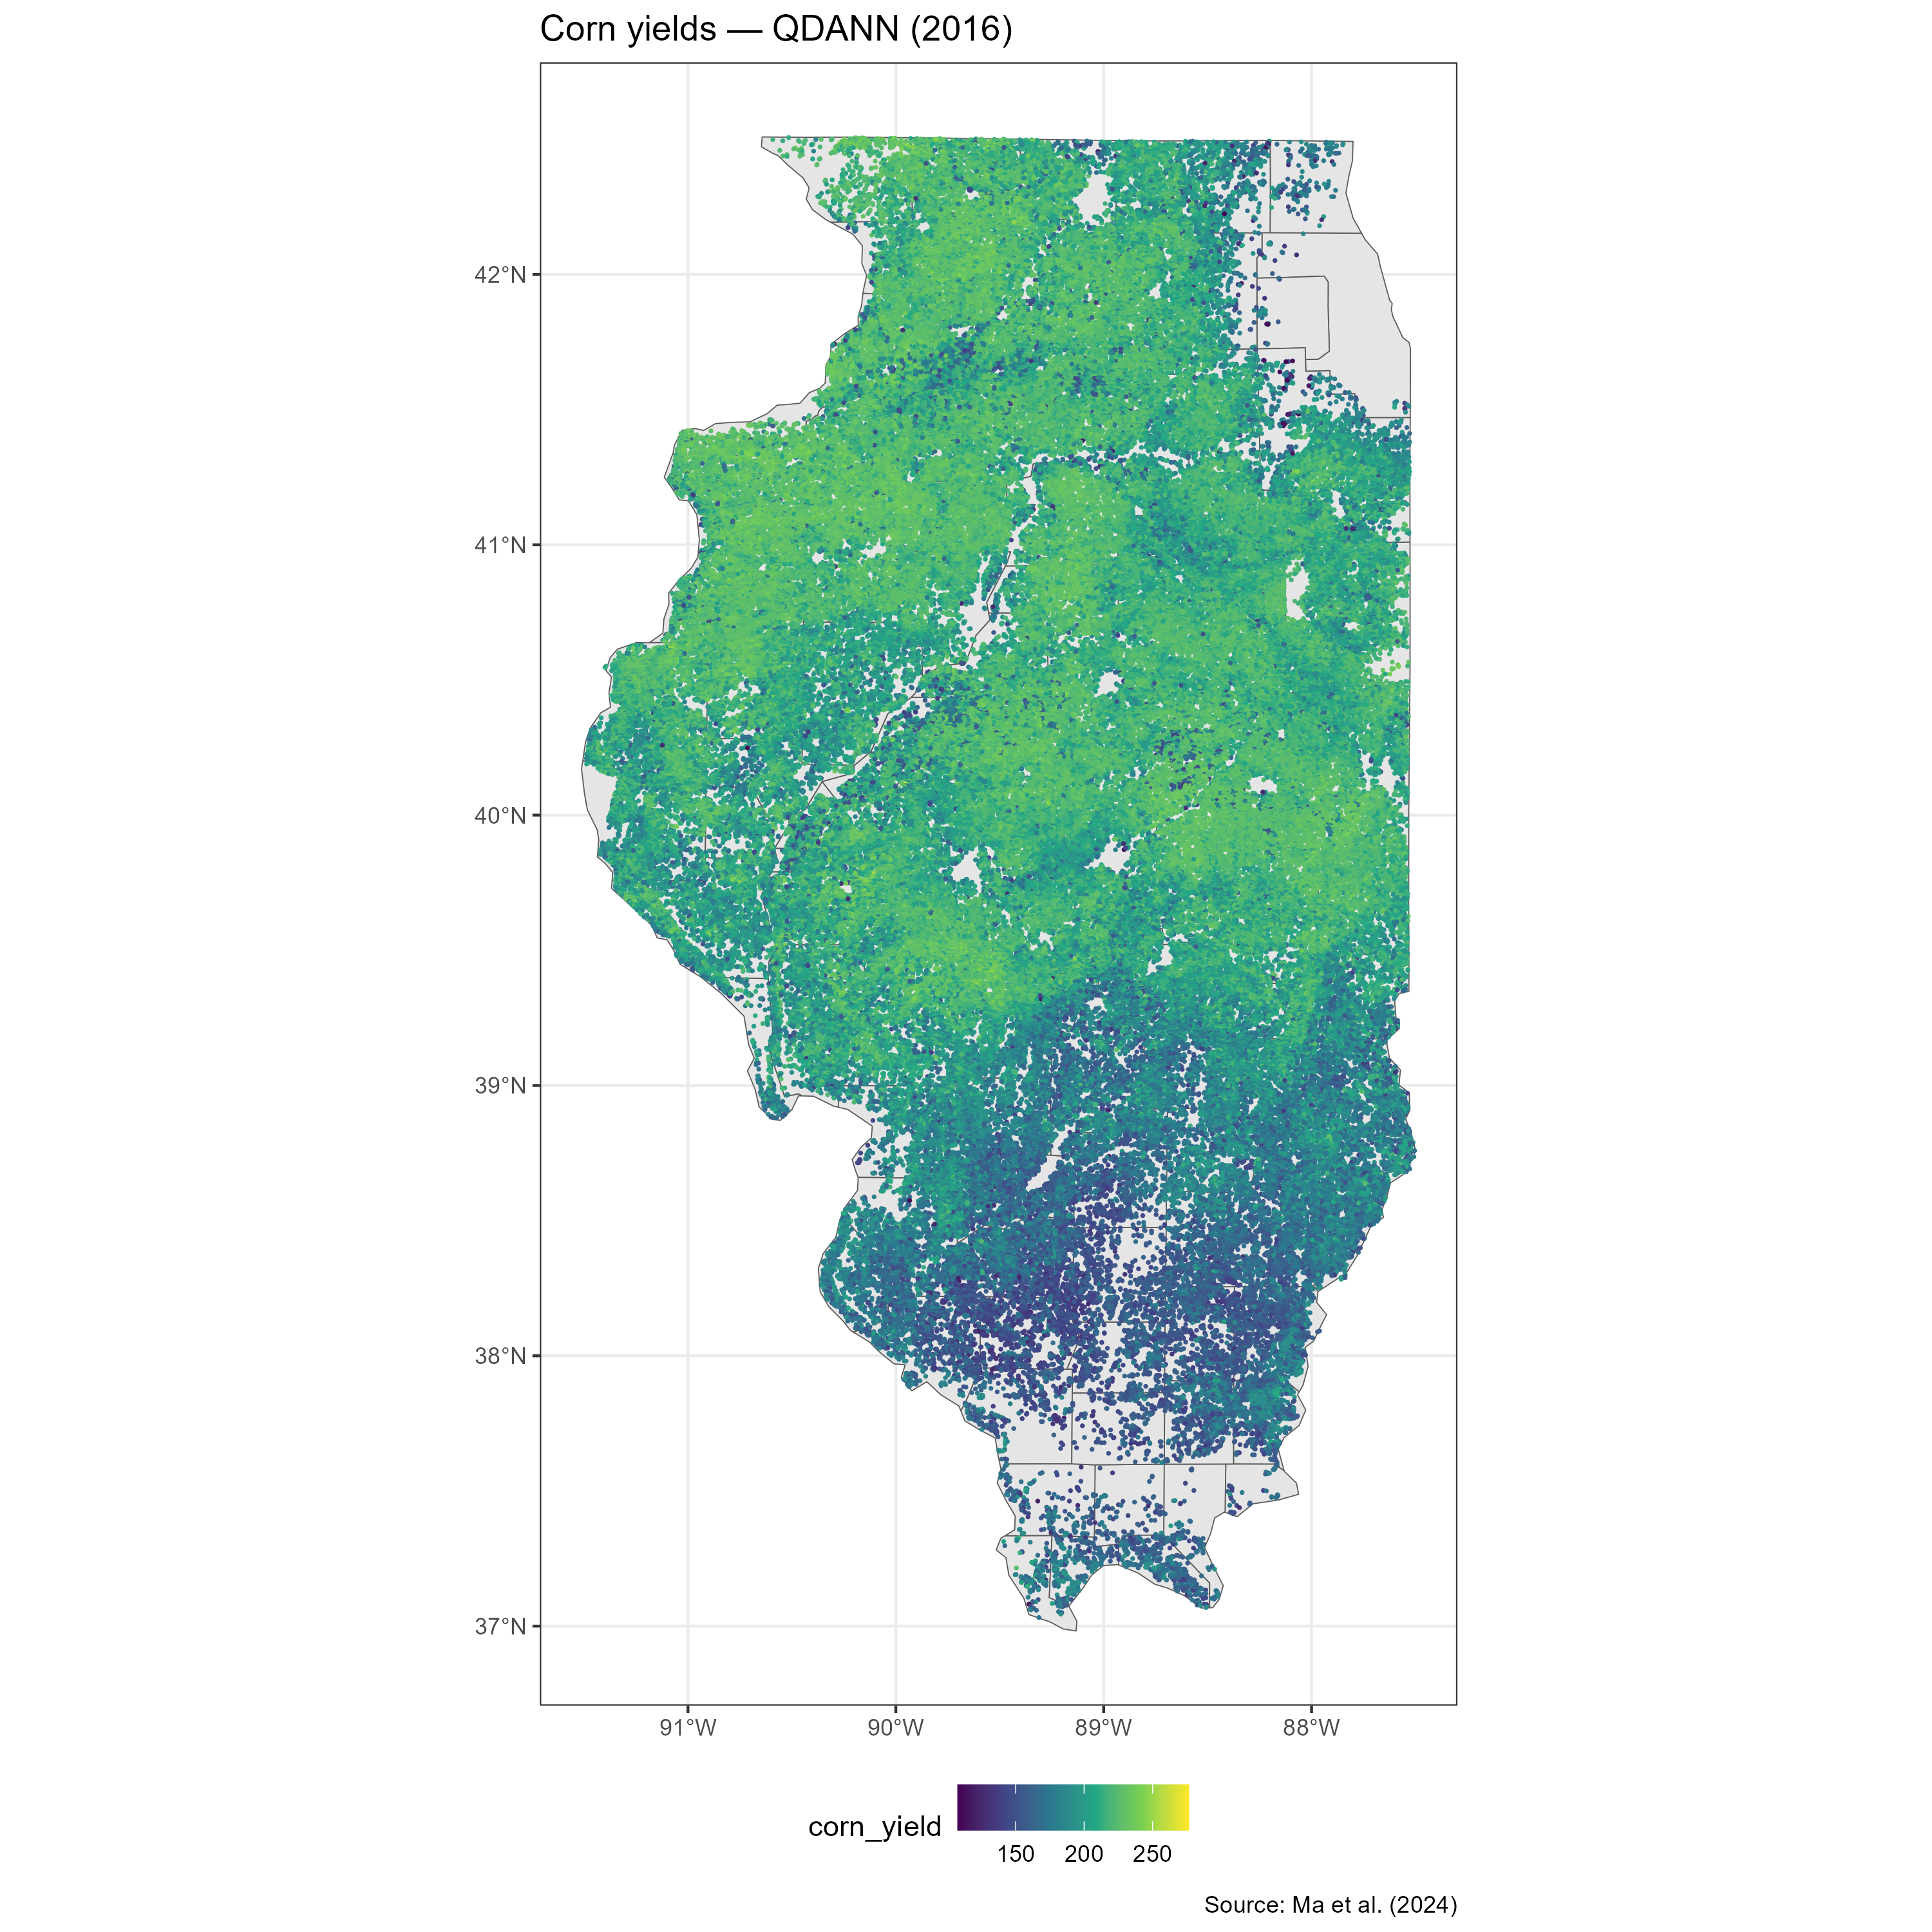
\includegraphics[width=0.85\textwidth]{figures/corn_yield_map}
  \caption{QDANN corn yields across Illinois, 2016.}
  \label{fig:corn_yield_map}
  \floatfoot{\footnotesize Notes: Spatial distribution of QDANN field-level corn
  yield estimates for Illinois in 2016. Source: \citet{Ma2024}.}
\end{figure}

\subsection{\label{subsec:rot_seq}Crop History and Rotation Sequences}
Field-level crop histories come from the USDA Cropland Data Layer \citep[CDL;][]{USDA2015}, an annual raster product produced by NASS that classifies each 30-meter pixel into a crop or land-cover category using satellite imagery and agricultural survey reference data. CDL has been available annually since 2008 for the full contiguous United States and since 2002 for Illinois. We use annual CDL data for Illinois from 2002 to 2022. The corn yield panel runs from 2008 to 2022 (15 outcome years); CDL classifications for 2002 to 2007 enter the analysis only as inputs to the six-year rotation histories of the earliest outcome years, so every outcome year has a complete six-year window.

For each field-pixel and outcome year $t$, we construct a six-year rolling rotation sequence by recording the CDL-classified crop in each of the years $t-1$ through $t-6$. Using the CDL numeric codes, we reclassify each year into one of three rotation crops: corn (code 1), soybean (code 5), and winter wheat (code 24). All remaining categories are treated as ``other.'' We restrict the analysis to field-year observations satisfying three conditions: corn is the outcome crop in year $t$; the six-year history contains only corn, soybean, or winter wheat, with no years classified as other crops, fallow, or non-agricultural land cover; and the field appears in at least two consecutive years in the panel after singleton removal. To keep the sequence space tractable and well supported, we further retain only the 29 distinct six-year sequences that together account for approximately 99\% of qualifying field-years, dropping rarer sequences observed in a negligible share of fields. After these restrictions, the qualifying corn sample contains 1,796,806 field-year observations for QDANN. Dropping the further 10,945 field-years with missing vapor pressure deficit leaves 1,785,861, and we estimate every field-level corn model reported in this paper (the sequence-effect, Just-Pope moment, Z-vector, and vapor-pressure-deficit specifications) on this common sample so that coefficients are comparable across tables.

We characterize rotation histories by the full sequence of crop codes over the six-year window. All retained sequences end in corn by the outcome restriction and enter the corn yield regressions as indicators relative to corn monoculture (coded $C-C-C-C-C-C$), giving 28 non-monoculture sequence effects; of these, 23 are pure corn-soybean sequences, and 5 contain at least one winter-wheat year. We refer to the latter as the corn-soybean-wheat system and separate the two systems in the sequence-effect figures. A companion paper summarizes rotation diversity instead using the Rotational Complexity Index (RCI) of \citet{socolar2021} and a set of mutually exclusive rotation regimes.

Two coding choices deserve note. First, winter wheat enters as a rotation-history covariate rather than as a modeled outcome: corn and soybean remain the outcome crops, and wheat appears only in the six-year predecessor window. Second, we initially considered extending the rotation set to alfalfa and to the winter-wheat/soybean double crop, both of which are agronomically distinct (alfalfa is a perennial nitrogen-fixing forage). In the Illinois sample, each accounts for well under one percent of field-years and does not appear in any of the 29 sequences clearing the 99\% support threshold used for the main sequence-dummy and Z-vector tables, so we restrict those analyses to corn, soybean, and winter wheat. The LASSO analysis in Section~\ref{subsec:lasso_results}, which considers a substantially larger unrestricted candidate set, does not recover any alfalfa-containing sequence for corn, consistent with alfalfa being too rare in this sample to identify a corn-side effect.

\subsection{\label{subsec:w_controls}Weather Controls}
We derive monthly precipitation totals, vapor pressure deficit (VPD), and a soil moisture index from GRIDMET \citep{Abatzoglou2013}, available at approximately 4-km spatial resolution. We aggregate each variable to monthly totals or means for June, July, and August. Following \citet{SchlenkerRoberts2009}, we replace monthly mean temperature with growing degree days (GDD) accumulated between 8\textdegree C and 29\textdegree C, and extreme degree days (EDD) accumulated above 29\textdegree C. Climate water deficit data come from TerraClimate \citep{Abatzoglou2018}.

\subsection{\label{subsec:soil_controls}Soil Controls}
Soil characteristics come from gSSURGO, produced by the USDA Natural Resources Conservation Service at 30-meter resolution. We extract three field-level measures: the National Commodity Crop Productivity Index (NCCPI), root-zone available water storage (AWC), and soil organic carbon stock (SOC) in the 0-100-centimeter depth zone. All three are field-level and effectively time-invariant, and are absorbed by the field fixed effects, so they are not separately identified once field fixed effects and the monthly soil-moisture controls are included; we therefore drop them from the preferred specification and retain the monthly soil-moisture terms.

\subsection{\label{subsec:smaple_const}Sample Construction and Summary Statistics}
We construct the estimation sample by merging the QDANN yield raster with CDL rotation sequences, GRIDMET and TerraClimate weather covariates, and gSSURGO soil variables at the 30-meter pixel level. The qualifying sample comprises 1,796,806 field-year observations; dropping field-years with missing vapor pressure deficit leaves 1,785,861, the common sample on which all field-level corn regressions reported below are estimated.

\begin{table}[!h]
\centering
\caption{\label{tab:corn_summary}Summary statistics by rotation type}
\centering
\resizebox{\ifdim\width>\linewidth\linewidth\else\width\fi}{!}{
\begin{tabular}[t]{lrrrrrrrr}
\toprule
Rotation type & N & Corn yield & RCI & Precip (Jun) & GDD (Jul) & EDD (Jul) & VPD (Jul) & AWC (mm)\\
\midrule
Corn monoculture & 154570 & 187.2 (33.2) & 0.00 (0.00) & 140.9 (70.2) & 409 (52) & 268.3 (2.8) & 1.19 (0.73) & 254 (46)\\
Perfect rotation & 996527 & 194.2 (31.1) & 2.24 (0.00) & 137.0 (67.4) & 420 (43) & 268.4 (2.2) & 1.05 (0.55) & 241 (45)\\
Transitioning & 287280 & 186.3 (33.5) & 1.82 (0.21) & 138.1 (67.8) & 412 (51) & 268.3 (2.7) & 1.16 (0.68) & 250 (45)\\
\bottomrule
\end{tabular}}
\end{table}

\vspace{-1ex}
\noindent{\footnotesize Notes: Means and standard deviations (in parentheses)
for QDANN corn yields and key covariates, by rotation type. Corn monoculture
= C-C-C-C-C-C; Perfect rotation = alternating C-S sequence; Transitioning =
sequences with RCI between 1.41 and 2.00.\par}

Table~\ref{tab:corn_summary} reports summary statistics for three illustrative rotation-type buckets within the corn sample (monoculture, the perfect alternating rotation, and transitioning sequences with RCI between 1.41 and 2.00) rather than the full sequence-dummy sample, so the reported $N$ sums to fewer observations than the full estimation sample. The pattern is consistent with the sequence-level results below: the perfect rotation bucket has both the highest mean yield (194.2 bu/acre) and the lowest yield standard deviation (31.1) of the three groups, while continuous corn has the lowest mean yield (187.2) and, together with the transitioning bucket, the highest variability (33.2 and 33.5, respectively).

Weather and soil covariates are broadly similar across rotation types within each crop, with the largest differences in June precipitation and growing degree days, consistent with rotation choice being only weakly correlated with the weather and soil controls once the sample is restricted to a single crop and county set; this supports the identification strategy in Section~\ref{subsec:stage_1}, which relies on within-field variation in rotation over time conditional on these same controls.

\section{Econometric Framework\label{sec:econ_framework}}
\subsection{\label{subsec:just_pope}The Just-Pope Framework and Its Variants}
The stochastic production function literature offers several approaches to jointly estimating the effects of inputs and management practices on the mean and variance of output. We briefly review the main variants to situate our estimator in the literature and motivate the specific implementation choices made here.

\medskip\noindent\textbf{Original two-stage OLS/FGLS - \cite{Just1978, Just1979}}.

Just and Pope proposed a general stochastic production specification of the form:

\begin{equation}
    y = f(\mathbf{X},\alpha)+\sqrt{h(\mathbf{X},\beta)}\times \varepsilon
\end{equation}

where $f(\cdot)$ is the conditional mean function and $h(\cdot)$ is the conditional variance function, both functions of the same input vector $\mathbf{X}$. This formulation relaxes the multiplicative stochastic restriction that dominated prior work - which
required inputs to be either uniformly risk-increasing or risk-neutral - and allows any input to raise or lower yield variance independently. From an econometric standpoint, the specification is a heteroskedastic regression model in which the variance of the production error is itself a function of inputs. The original estimation procedure uses two stages: OLS of the mean function to recover residuals, then OLS (or NLS for nonlinear mean functions) of the squared residuals on the variance function covariates.

\medskip\noindent\textbf{Antle's flexible moment-based extension - \cite{antle1983, Antle2010}}.

\cite{antle1983} extended the Just-Pope framework to estimate higher moments of the output distribution beyond the mean and variance, showing that the first three moments of milk yield are statistically significant functions of inputs. This matters for
insurance applications because indemnities depend on left-tail probabilities, and mean-variance summaries may miss important skewness effects. \cite{Antle2010} later proposed partial-moment functions as a flexible way to characterize asymmetric input effects on output distributions. We implement the third-moment case of this extension for corn: alongside the stage-1 mean and stage-2 variance equations, we estimate a third-stage moment regression of the cubed first-stage residual on the same rotation-sequence and control variables, recovering the effect of each sequence on the conditional skewness of corn yields (Table~\ref{tab:corn_jp_moments}). Because low-yield realizations trigger indemnities, this third moment is the distributional margin most directly relevant to insurance pricing. \citet{difalco2009} apply this moment-based approach to crop diversity in Ethiopian agriculture and find that greater diversity reduces both production variance and downside-risk exposure. Their diversity measure is cross-sectional, the mix of crops grown in a given season, rather than the temporal rotation we study, so whether an analogous downside-risk benefit carries over to field-scale corn rotations in the US Corn Belt is an open empirical question, and one we take up directly in Section~\ref{subsec:var_effects}.

\medskip\noindent\textbf{Maximum likelihood and log-linear variance - \cite{Harvey1976, Saha1997}}.

Researchers have traditionally estimated Just-Pope functions using feasible generalized least squares (FGLS). \cite{Saha1997} use Monte Carlo experiments showing that, in small samples, even when the error distribution departs from normality, the maximum likelihood (ML) estimator is more efficient and less biased than FGLS, and that FGLS can seriously understate the risk effects of inputs. A related improvement is the log-linear variance specification proposed by \cite{Harvey1976}, which replaces the linear regression of $\hat{\varepsilon}^2$ on $\mathbf{X}$ with a regression of $\log \hat{\varepsilon}^2$ on $\mathbf{X}$, then exponentiates fitted values to obtain strictly positive variance estimates. This avoids the truncation problem that arises when the linear approximation produces negative fitted values for some cells. We implement the three-stage FGLS estimator with a linear variance specification and
address the truncation problem by flooring negative fitted values at a small positive constant (see Section~\ref{subsec:stage_2}); we report the log-linear specification as a robustness check.

\medskip\noindent\textbf{Joint estimation with risk preferences and technical efficiency - \cite{Kumbhakar2002}}.

\cite{Kumbhakar2002} embeds the Just-Pope variance function inside a stochastic frontier model, jointly estimating production risk, risk preferences, and technical inefficiency without imposing parametric restrictions on the utility function. A limitation of the standard Just-Pope formulation is that it does not account for producers' preferences, so that input elasticities are treated as invariant to risk perceptions. Kumbhakar's extension addresses this at the cost of additional distributional assumptions on the inefficiency term. We do not pursue this extension here, as our primary interest is in the population distribution of rotation effects rather than in individual farm efficiency.

\medskip\noindent\textbf{Nonparametric extension - \cite{li2021}}.

The most flexible variant in the recent literature is the nonparametric production risk estimator of \cite{li2021}, in which both the mean function $f(\cdot)$ and the variance function $h(\cdot)$ are estimated using local polynomial regression rather than parametric functional forms. This allows the risk effect of any variable to vary continuously with a conditioning covariate - for example, the variance effect of a recent soybean placement varying smoothly with soil productivity. The LRZ estimator nests the parametric Just-Pope model as a special case in which the local polynomial slopes are constant. We implement the parametric Just-Pope estimator as our main specification and the LRZ nonparametric extension as a robustness check, allowing rotation effects to vary with NCCPI soil productivity, following the approach described in Section 4 of \cite{li2021}.

Our main estimator follows the three-stage FGLS approach of \cite{Harvey1976} and \cite{Saha1997}, embedded in a panel fixed effects framework with two-way clustering for inference. We describe the specific implementation in Sections~\ref{subsec:stage_1} through~\ref{subsec:bootstrap} below.

\subsection{\label{subsec:stage_1}Conditional Mean: Stage 1}
We model the conditional mean of corn yields as a two-way fixed effects regression following the linear panel framework:

\begin{equation}
    y_{it}=\text{seq}_{it}'\tau+ W_{it}'\beta+\lambda_{i}+\gamma_{t}+\varepsilon_{it}\label{eq:stage1}
\end{equation}

where $y_{it}$ is the yield of field $i$ year $t$ measured in bushels per acre; $\text{seq}_{it}$ is a vector of rotation sequence indicators, with corn monoculture as the reference category; $W_{it}$ is a vector of weather and soil controls described in Section~\ref{subsec:w_controls}; $\lambda_{i}$ is a field ($\text{tile\_field\_ID}$) fixed effect; and $\gamma_{t}$ is a year fixed effect. The error term $\varepsilon_{it}$ is assumed to
have a conditional mean of zero given the regressors.

Field fixed effects absorb all time-invariant differences across fields in average yield levels, including persistent soil quality, drainage, and field-specific management. Year fixed effects absorb common shocks to all fields in a given year, including statewide weather events and aggregate commodity price signals that affect input use uniformly. Identification of the rotation effect $\hat{\tau}$ therefore comes from within-field variation in rotation sequences over time, conditional on the weather and soil controls, so only fields that change rotation pattern during the panel contribute. Standard errors are clustered two-way at the county ($\text{COUNTY\_FIPS}$) and year levels, following \cite{Cameron2015}, to account for arbitrary within-county correlation (including serial correlation within fields) and for common shocks across fields in the same growing season.

\medskip\noindent\textbf{LASSO selection of rotation sequences}. Rather than summarizing the rotation feature space with an unsupervised technique such as PCA, we let the outcome data itself determine which six-year sequences carry independent information about yields. We do this in three steps.

First, we partial out field and year fixed effects from both the outcome and every candidate sequence indicator via the Frisch-Waugh-Lovell (FWL) theorem, using the same demeaning procedure the \texttt{fixest} R package uses internally for equation~\eqref{eq:stage1}. This is necessary, not merely convenient: with field fixed effects at the tile-field level, including field dummies directly as LASSO regressors would be both computationally infeasible and statistically incorrect, since the penalty would shrink the fixed effects along with everything else and reintroduce the within-field confounding that the fixed-effects design is meant to remove. Weather and soil controls are partialled out in the same step, so that a selected sequence reflects rotation-specific yield variation rather than the growing conditions correlated with where that rotation happens to be planted.

Second, we regress the demeaned outcome on the demeaned sequence indicators using LASSO, which shrinks coefficients on sequences with little independent explanatory power for yield exactly to zero rather than merely toward zero, so it performs variable selection rather than only shrinkage. We use the plug-in penalty of \citet{Belloni2014} as implemented in \texttt{rlasso}, which is heteroskedasticity-robust and does not require cross-validation to tune. Formally, with $\tilde{y}_{it}$ and $\tilde{\text{seq}}_{it}$ denoting the field- and year-demeaned outcome and sequence-indicator vector,
%
\begin{equation}
  \hat{\tau}^{\text{LASSO}} = \operatorname*{arg\,min}_{\tau} \; \frac{1}{N}\sum_{it}\left(\tilde{y}_{it} - \tilde{\text{seq}}_{it}'\tau\right)^2 + \frac{\lambda}{N}\sum_{k}\psi_k|\tau_k|
  \label{eq:lasso}
\end{equation}
%
where $\lambda$ is the plug-in penalty level and $\psi_k$ are data-dependent penalty loadings that adjust for heteroskedasticity across sequences.

Third, because the $\ell_1$ penalty in equation~\eqref{eq:lasso} biases the surviving coefficients toward zero and does not admit standard errors in the usual sense, we treat the LASSO step as a variable-selection device only. We refit an unpenalized fixed-effects regression, in the form of equation~\eqref{eq:stage1}, restricted to the sequences with nonzero $\hat{\tau}^{\text{LASSO}}_k$, with the same two-way clustered standard errors used throughout the paper. This two-stage procedure, using LASSO for selection and ordinary least squares for estimation and inference on the selected model, follows \citet{Belloni2014} and ensures that the coefficients and significance levels we report are not mechanically shrunk or otherwise affected by selection.

Of the 102 candidate corn sequences considered (the unrestricted sample, before any 99\%-frequency cut), 29 have nonzero post-selection coefficients (28.4\%). Full post-selection refit coefficients are reported in Table~\ref{tab:corn_lasso}, discussed in Section~\ref{subsec:lasso_results}.


We also estimate a parsimonious parameterization that replaces the sequence indicators with three structural rotation features:
%
\begin{equation}
  y_{it} = Z_{it}'\tau + W_{it}'\beta + \lambda_i + \gamma_t + \varepsilon_{it}
  \label{eq:zvector}
\end{equation}
%
 Where $Z_{it} = [\text{late\_soy}_{it},\ \text{soy\_cons}_{it},\ \text{soy\_gap}_{it}]$: the soy lag, a consecutive-soy dummy, and the minimum gap between soybean harvests. We code $\text{late\_soy}$ as a non-positive integer running from $-6$ to $0$, equal to minus the number of years since the most recent soybean harvest ($-1$ if soybean was grown in year $t-1$, $-6$ if the only soybean year is $t-6$, and $0$ for monoculture windows with no soybean year); values closer to zero therefore denote a more recent soybean harvest, so a positive coefficient means that greater soybean recency raises corn yield. We initially also included the total number of soybean harvests in the window ($\text{nsoy}$), but it is strongly collinear with the soybean-gap feature (correlation $0.65$), which rendered its coefficient unstable across specifications; we therefore drop it and let the gap feature carry the soybean-frequency signal. The three retained features are close to orthogonal (pairwise correlations below $0.17$ in absolute value).

Because the 28 sequence indicators are tested simultaneously against the monoculture reference, we report \cite{Benjamini1995} false discovery rate-adjusted p-values alongside unadjusted p-values in Table~\ref{tab:corn_rot}. The parsimonious Z-vector model in Table~\ref{tab:zvector} is our confirmatory specification with three pre-specified hypotheses; we treat the sequence-level results as exploratory.

\subsection{\label{subsec:stage_2}Conditional Variance: Stage 2 (Just-Pope Framework)}

To separately identify the effect of rotations on yield risk, we follow \cite{Just1979} and \cite{antle1983} in estimating a second-stage regression of squared first-stage residuals on the same regressors. Let $\hat{u}_{it} = y_{it}-\hat{y}_{it}$ denote
the residual from the stage-1 conditional mean regression. The second moment is then estimated as:

\begin{equation}
    \hat{u}_{it}^2 = \text{seq}_{it}'\pi + W_{it}'\delta + \lambda_i + \gamma_t + \nu_{it}\label{eq:stage2}
\end{equation}

Coefficients $\hat{\pi}$ identify the differential effect of each rotation sequence on the conditional variance of yields, relative to the monoculture reference. A negative coefficient indicates that a given sequence compresses yield variance relative to monoculture - a risk-reducing effect directly relevant to insurance pricing. A positive coefficient indicates that the sequence raises variance, increasing actuarial risk at any given mean yield level.

The squared residual $\hat{u}_{it}^2$ is a noisy proxy for the true conditional variance, since it combines the variance signal with idiosyncratic estimation error from stage 1. To improve estimation efficiency, we implement a three-stage Feasible Generalized Least Squares (FGLS) estimator following \cite{Harvey1976}. In stage 2a, we estimate an initial OLS regression of $\hat{u}_{it}^2$ on the full set of covariates to obtain fitted values $\hat{h}_{it}$, which serve as estimates of the conditional variance function. In stage 2b, we re-estimate the variance regression by Weighted Least Squares (WLS), weighting each observation by $1/\hat{h}_{it}$ where $\hat{h}_{it}= \max(\hat{h}_{it}^{\text{OLS}},\ \varepsilon)$ with $\varepsilon = 10^{-6}$ to prevent degenerate weights from negative linear approximations to the variance function. The FGLS estimator is more efficient than the OLS second-stage estimator because it downweights observations whose squared residuals are expected to be highly variable - those from rotation sequences with high estimated conditional variance.

\subsection{\label{subsec:bootstrap}Inference: Three-Stage Bootstrap}

Both the OLS and FGLS stage-2 estimators face a generated-regressor problem: the dependent variable $\hat{u}_{it}^2$ is constructed from first-stage estimates and therefore contains estimation error that standard second-stage standard errors do not account for. In the FGLS case, the weights $\hat{h}_{it}$ are themselves estimated, introducing a third source of uncertainty. We address the generated-regressor problem for both estimators by implementing a pairs cluster bootstrap that wraps all three stages and propagates first-stage uncertainty through to the final variance estimates.

The bootstrap procedure proceeds as follows. In each of $B = 999$ iterations, we draw a bootstrap sample by resampling $n$ fields with replacement from the $n$ unique fields in the estimation sample, where the bootstrap weight of field $j$ equals the number of times it was drawn. Rather than physically duplicating rows - which, at approximately 1.55 million observations, would exhaust available memory - we implement a frequency-weighted bootstrap that assigns each field a bootstrap weight equal to its draw count and passes this weight to all three estimation stages via the \texttt{weights} argument of the regression function. Fields not drawn receive weight zero and are excluded from that iteration. Within each iteration, stages 1, 2a, and 2b are re-estimated on the weighted sample, and the stage-2b coefficient vector is stored. Bootstrap standard errors are computed as the standard deviation of the stored coefficient draws across $B$ iterations, and 95 percent confidence intervals are constructed as the 2.5th and 97.5th percentiles of the bootstrap distribution. We maintain all fixed effects and clustering within each bootstrap iteration.

This bootstrap design has two important properties. First, by resampling at the field level, it respects the within-field serial correlation in the panel - all years of a given field enter the bootstrap sample together or not at all. Second, by wrapping all
three stages in a single loop, the bootstrap correctly accounts for the covariance between the stage-1 residuals and the stage-2 weights, which a naive two-step bootstrap that treats stage-1 as fixed would miss.

\subsection{\label{subsec:rot_score}Rotation Score}
The three structural feature coefficients from the parsimonious stage-1 model admit a natural rotation scoring rule. For each field-year observation, we define the rotation score as:

\begin{equation}
    \text{score}_{it} = \hat{\tau}_1 \cdot \text{late\_soy}_{it} + \hat{\tau}_2 \cdot \text{soy\_cons}_{it} + \hat{\tau}_3 \cdot \text{soy\_gap}_{it}\label{eq:score}
\end{equation}

where $\hat{\tau}_1, \hat{\tau}_2, \hat{\tau}_3$ are the QDANN stage-1 estimates from Table~\ref{tab:zvector}. The score summarizes, in units of predicted yield deviation from monoculture, the information contained in the six-year rotation history relevant to the conditional mean of corn yields. By construction, corn monoculture, which has no soybean years in the window, scores zero.

Rotation sequences that score below zero have structural features that are predicted to lower mean yields relative to continuous corn; these sequences typically involve multiple consecutive soybean years or very infrequent soybean harvests that deplete
the nitrogen and pest-suppression benefits of rotation. Sequences that score above zero have structural features associated with higher mean yields, particularly a recent soybean harvest and adequate spacing between soybean years.

\section{\label{sec:results}Results}
\subsection{\label{subsec:seq_effects}Sequence-Level Effects on Corn Yield Mean}

Table~\ref{tab:corn_rot} and Figure~\ref{fig:corn_rot_plot} report the estimated effects of each of the 28 non-monoculture six-year sequences on the mean corn yield, relative to corn monoculture. Of the 28, 23 are pure corn-soybean sequences, and 5 contain at least one winter-wheat year; Figure~\ref{fig:corn_rot_plot} separates the two systems into panels. Rotation effects are heterogeneous and depend on the recent history of soybean placement rather than on the total number of soybean years in the window. The winter-wheat sequences are estimated on substantially thinner support and carry wider confidence intervals, so the contrast between the two panels reflects precision as much as agronomy.


\begin{table}[H]
   \caption{\label{tab:corn_rot} Rotation patterns and corn yields}
   \bigskip
   \centering
   \scriptsize
   \renewcommand*{\arraystretch}{0.8}
   \begin{tabular}{lcc}
      \toprule
       & \multicolumn{2}{c}{corn\_yield}\\
                                      & No controls              & With controls \\   
                                      & (1)                      & (2)\\  
      \midrule 
      W-C-C-S-W-C                     & 8.329$^{***}$ (1.537) [p<0.001]    & 7.630$^{***}$ (1.496) [p<0.001]\\   
      C-S-C-W-S-C                     & 8.170$^{***}$ (1.492) [p<0.001]    & 6.311$^{***}$ (1.368) [p<0.001]\\   
      S-S-C-S-S-C                     & 6.861$^{***}$ (0.5615) [p<0.001]   & 5.938$^{***}$ (0.5157) [p<0.001]\\   
      C-C-C-S-W-C                     & 6.826$^{***}$ (0.6815) [p<0.001]   & 5.810$^{***}$ (0.6512) [p<0.001]\\   
      S-C-S-W-S-C                     & 6.292$^{***}$ (0.6945) [p<0.001]   & 5.772$^{***}$ (0.6868) [p<0.001]\\   
      C-S-C-S-S-C                     & 5.430$^{***}$ (0.4847) [p<0.001]   & 4.824$^{***}$ (0.4312) [p<0.001]\\   
      S-S-S-S-S-C                     & 5.061$^{***}$ (0.6902) [p<0.001]   & 4.655$^{***}$ (0.5542) [p<0.001]\\   
      S-C-S-S-S-C                     & 5.270$^{***}$ (0.5453) [p<0.001]   & 4.609$^{***}$ (0.4616) [p<0.001]\\   
      C-C-C-C-S-C                     & 4.628$^{***}$ (0.3541) [p<0.001]   & 4.411$^{***}$ (0.3639) [p<0.001]\\   
      S-S-C-C-S-C                     & 5.004$^{***}$ (0.5438) [p<0.001]   & 4.308$^{***}$ (0.5122) [p<0.001]\\   
      C-S-S-S-S-C                     & 4.305$^{***}$ (0.6044) [p<0.001]   & 4.284$^{***}$ (0.5434) [p<0.001]\\   
      S-C-C-C-S-C                     & 4.696$^{***}$ (0.3683) [p<0.001]   & 4.230$^{***}$ (0.3499) [p<0.001]\\   
      S-C-C-S-W-C                     & 5.012$^{***}$ (0.7216) [p<0.001]   & 4.121$^{***}$ (0.6876) [p<0.001]\\   
      C-S-C-C-S-C                     & 4.494$^{***}$ (0.3984) [p<0.001]   & 4.089$^{***}$ (0.3658) [p<0.001]\\   
      C-C-S-C-S-C                     & 4.286$^{***}$ (0.4121) [p<0.001]   & 4.071$^{***}$ (0.3928) [p<0.001]\\   
      C-C-C-S-S-C                     & 3.602$^{***}$ (0.5559) [p<0.001]   & 3.746$^{***}$ (0.5121) [p<0.001]\\   
      S-C-S-C-S-C                     & 4.195$^{***}$ (0.4310) [p<0.001]   & 3.632$^{***}$ (0.3953) [p<0.001]\\   
      S-C-C-S-S-C                     & 3.943$^{***}$ (0.6356) [p<0.001]   & 3.287$^{***}$ (0.5725) [p<0.001]\\   
      S-S-S-C-S-C                     & 3.650$^{***}$ (0.5843) [p<0.001]   & 3.250$^{***}$ (0.5012) [p<0.001]\\   
      C-C-C-S-C-C                     & 2.463$^{***}$ (0.2341) [p<0.001]   & 2.105$^{***}$ (0.2482) [p<0.001]\\   
      C-S-C-S-C-C                     & 1.436$^{***}$ (0.3704) [p<0.001]   & 1.028$^{***}$ (0.3617) [p=0.005]\\   
      S-C-S-S-C-C                     & 1.214$^{**}$ (0.5779) [p=0.038]    & 0.6850 (0.5368) [p=0.205]\\   
      C-C-S-C-C-C                     & 0.9810$^{***}$ (0.2932) [p=0.001]  & 0.6844$^{**}$ (0.2820) [p=0.017]\\   
      S-C-S-C-C-C                     & 0.9022$^{***}$ (0.3191) [p=0.006]  & 0.4936 (0.3144) [p=0.119]\\   
      S-S-C-S-C-C                     & 0.0523 (0.6005) [p=0.931]          & -0.6638 (0.5569) [p=0.236]\\   
      C-S-C-C-C-C                     & -0.6166$^{**}$ (0.2826) [p=0.031]  & -0.7695$^{***}$ (0.2520) [p=0.003]\\   
      S-C-C-C-C-C                     & -0.7831$^{***}$ (0.2424) [p=0.002] & -1.076$^{***}$ (0.2311) [p<0.001]\\   
      S-S-C-C-C-C                     & -1.096 (0.7090) [p=0.125]          & -1.326$^{**}$ (0.6373) [p=0.040]\\   
       \\
      Observations                    & 1,796,806                & 1,796,806\\  
      R$^2$                           & 0.81623                  & 0.84354\\  
      Within R$^2$                    & 0.00690                  & 0.15452\\  
      Controls                        & No                       & Yes\\  
       \\
      tile\_field\_ID fixed effects   & $\checkmark$             & $\checkmark$\\   
      year fixed effects              & $\checkmark$             & $\checkmark$\\   
      \bottomrule
   \end{tabular}
\end{table}



\begin{quote}
\small
Notes: Dependent variable is QDANN corn yield in bushels per acre. Reference category: corn monoculture (C-C-C-C-C-C). Column (1) excludes weather and soil controls; column (2) includes full control vector. Field (tile\_field\_ID) and year fixed effects are included throughout; standard errors are two-way clustered at county and year. Stars indicate BH-FDR adjusted significance: $^{***}$FDR$<$0.01, $^{**}$FDR$<$0.05, $^{*}$FDR$<$0.10.
\end{quote}

\begin{figure}[H]
  \centering
  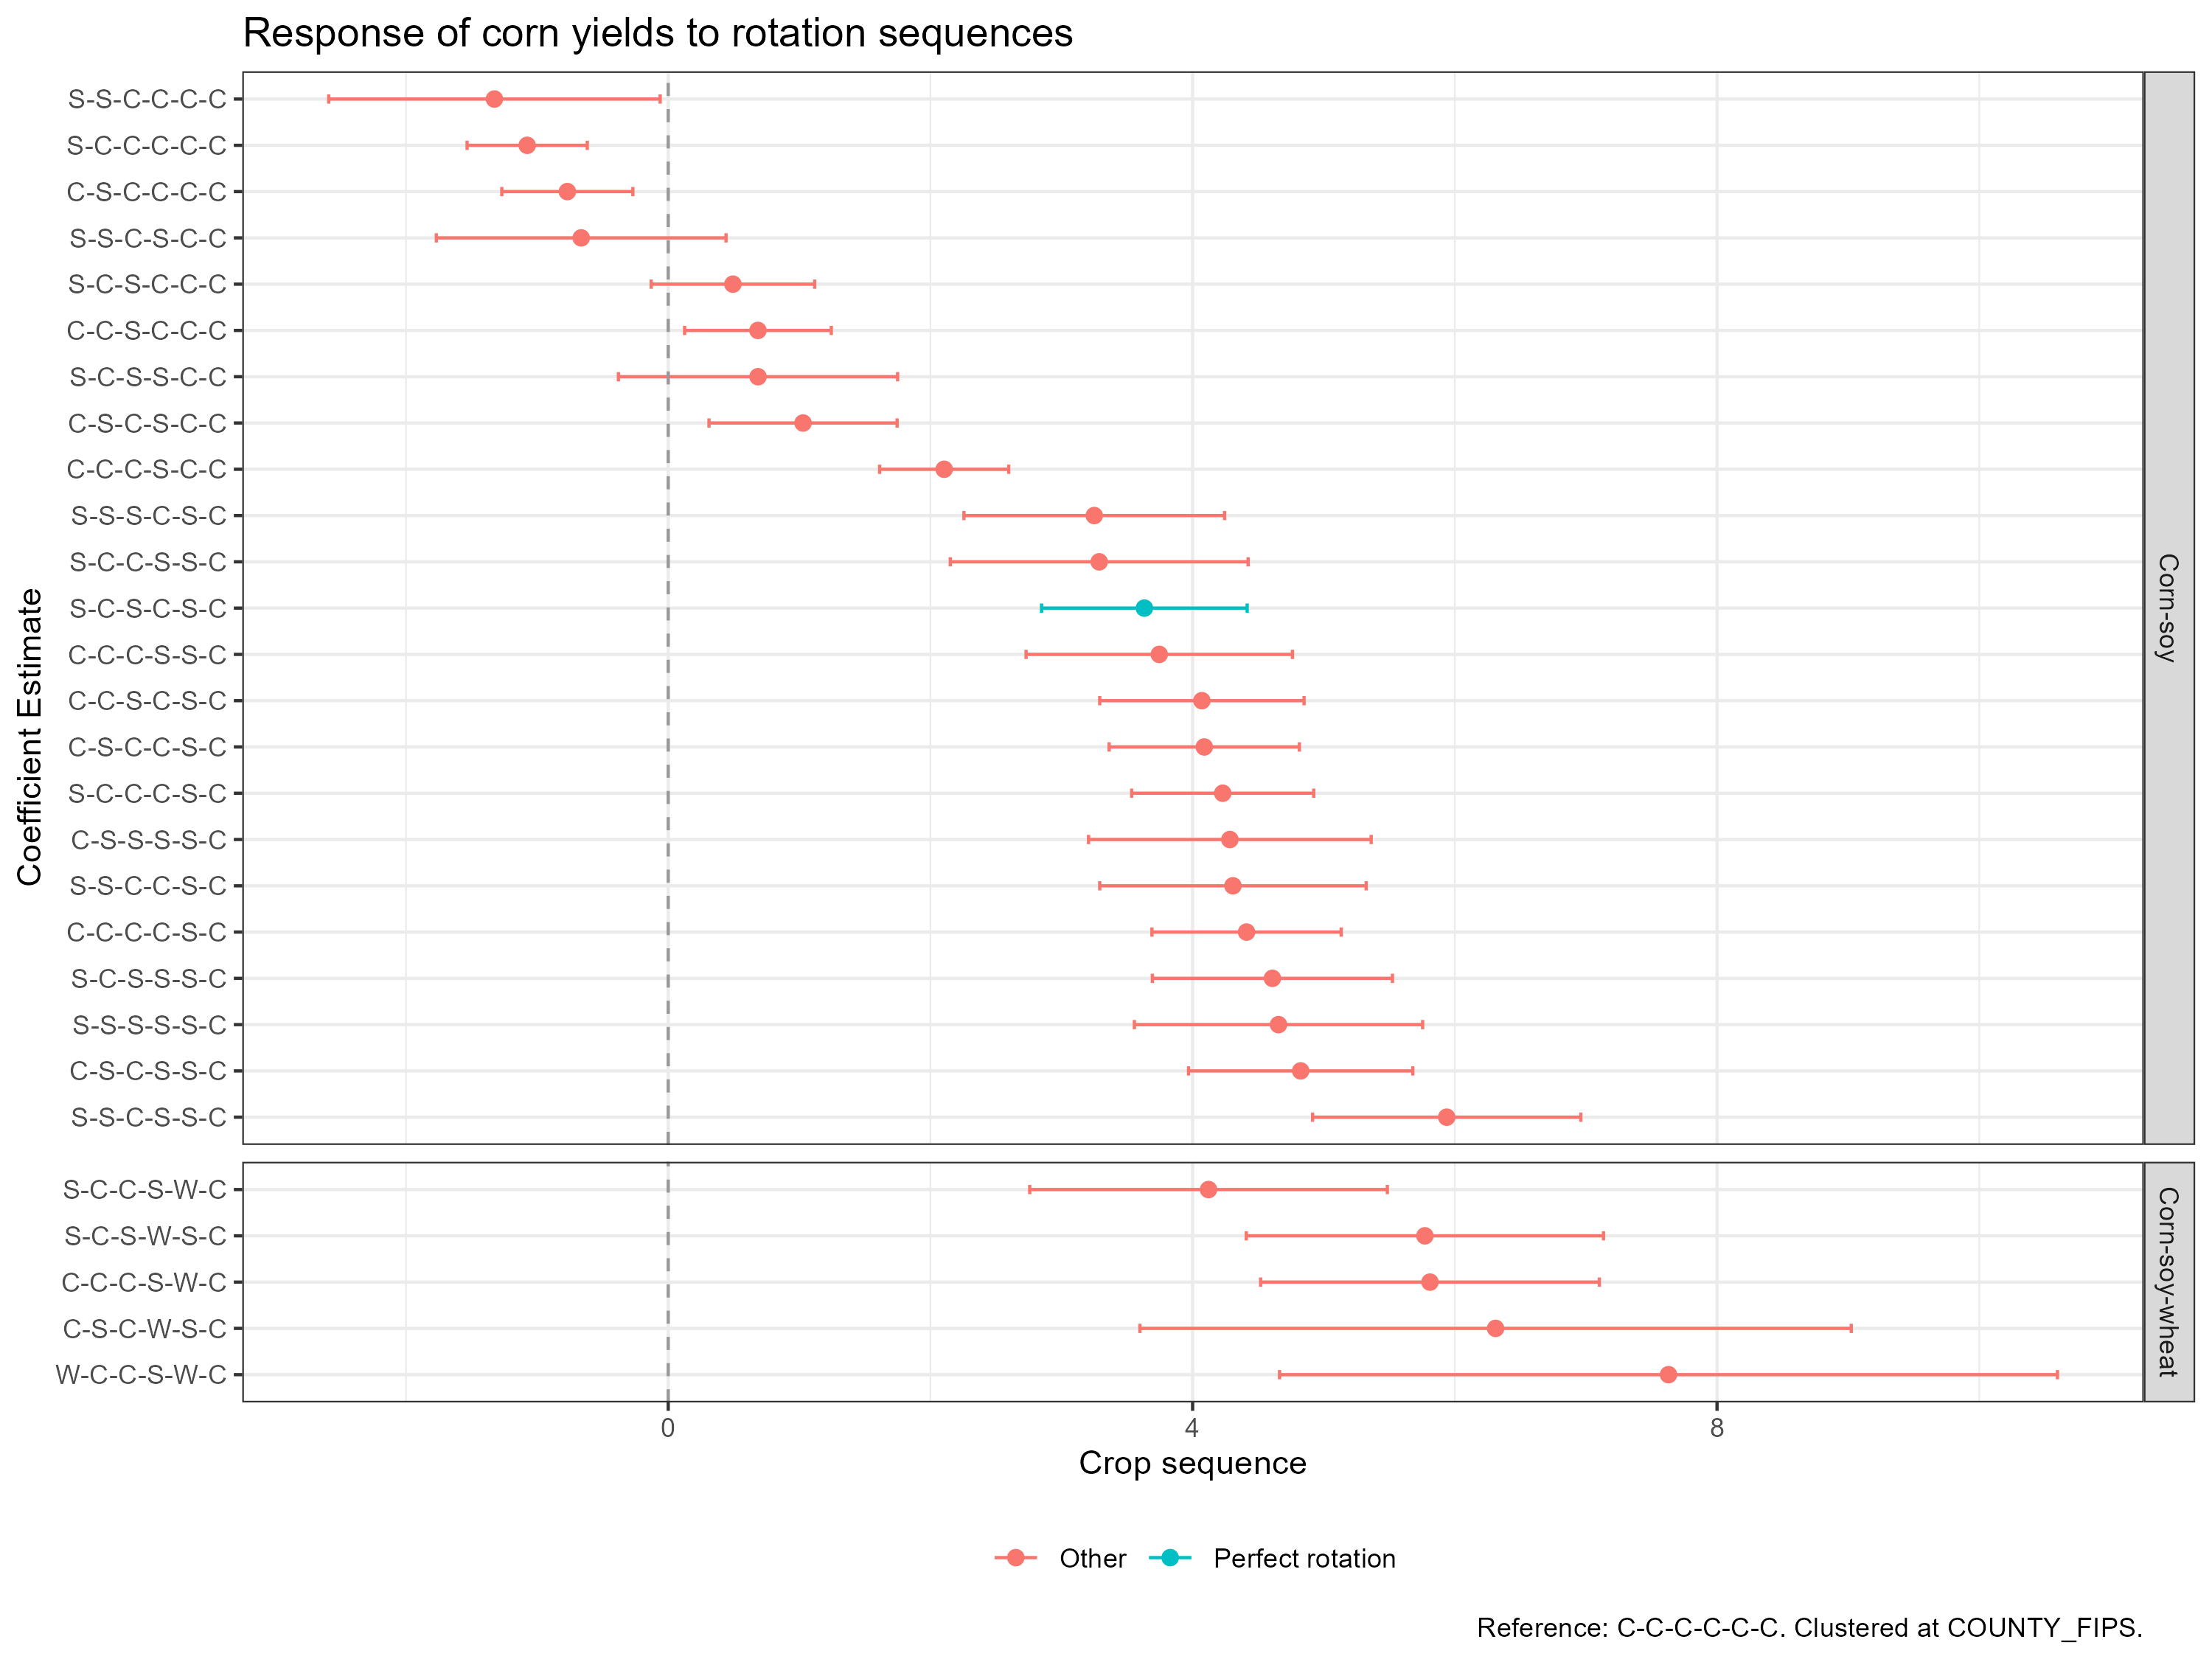
\includegraphics[width=0.90\textwidth]{figures/corn_rot_plot}
  \caption{Response of corn yields to rotation sequences.}
  \label{fig:corn_rot_plot}
  \floatfoot{\footnotesize Notes: Point estimates and 95\% confidence intervals
  from equation~\eqref{eq:stage1} with full controls. Reference: corn monoculture
  (C-C-C-C-C-C). Two-way clustering at county and year level. Green: perfect
  alternating rotation; blue: transitioning sequences; red: all others.}
\end{figure}


The highest-performing sequences in the QDANN specification-those with estimated mean yield premiums exceeding 4 bushels per acre-share a common structural feature: a soybean harvest in year $t-1$ or $t-2$, regardless of what was planted in years $t-3$ through $t-6$. For example, $S-S-C-S-S-C$ carries an estimated premium of 5.94 bushels per acre relative to monoculture (Table~\ref{tab:corn_rot}, column 2), and $C-S-C-S-S-C$ carries 4.82 bushels per acre.

Sequences ending in two or more consecutive corn years generally show negative or near-zero coefficients. The two continuous-corn-adjacent sequences $C-S-C-C-C-C$ and $S-C-C-C-C-C$ carry negative mean effects in the full specification, at $-0.77$ ($p<0.10$) and $-1.07$ ($p<0.05$) bushels per acre respectively. The perfect alternating corn-soybean rotation ($S-C-S-C-S-C$) carries a positive and statistically significant coefficient of approximately $3.64$ bushels per acre; a single well-placed recent soybean does even better, however: $C-C-C-C-S-C$ reaches $4.42$ bushels per acre, indicating that the rotation benefit materializes primarily through the most recent soybean placement rather than through sustained alternation.

\subsection{\label{subsec:var_effects}Sequence-Level Effects on Corn Yield Variance}

Figure~\ref{fig:corn_var_plot} and the full stage-2 variance results (Table~\ref{tab:corn_jp_moments}, Appendix) show the corresponding effects on the conditional variance of corn yields; because the conditional-variance estimators are secondary to the mean results in this setting, the sequence-by-sequence coefficient table is reported in the Appendix rather than the main text. Sequences that raise mean yields also tend to reduce yield variance, implying joint mean-variance dominance over monoculture. Sequences with a very recent soybean placement (year $t-1$) tend to show negative variance coefficients; $C-C-C-C-S-C$, for example, carries a marginally significant variance reduction ($-2.6$, $p<0.10$; Table~\ref{tab:corn_jp_moments}, Appendix).

\begin{figure}[H]
  \centering
  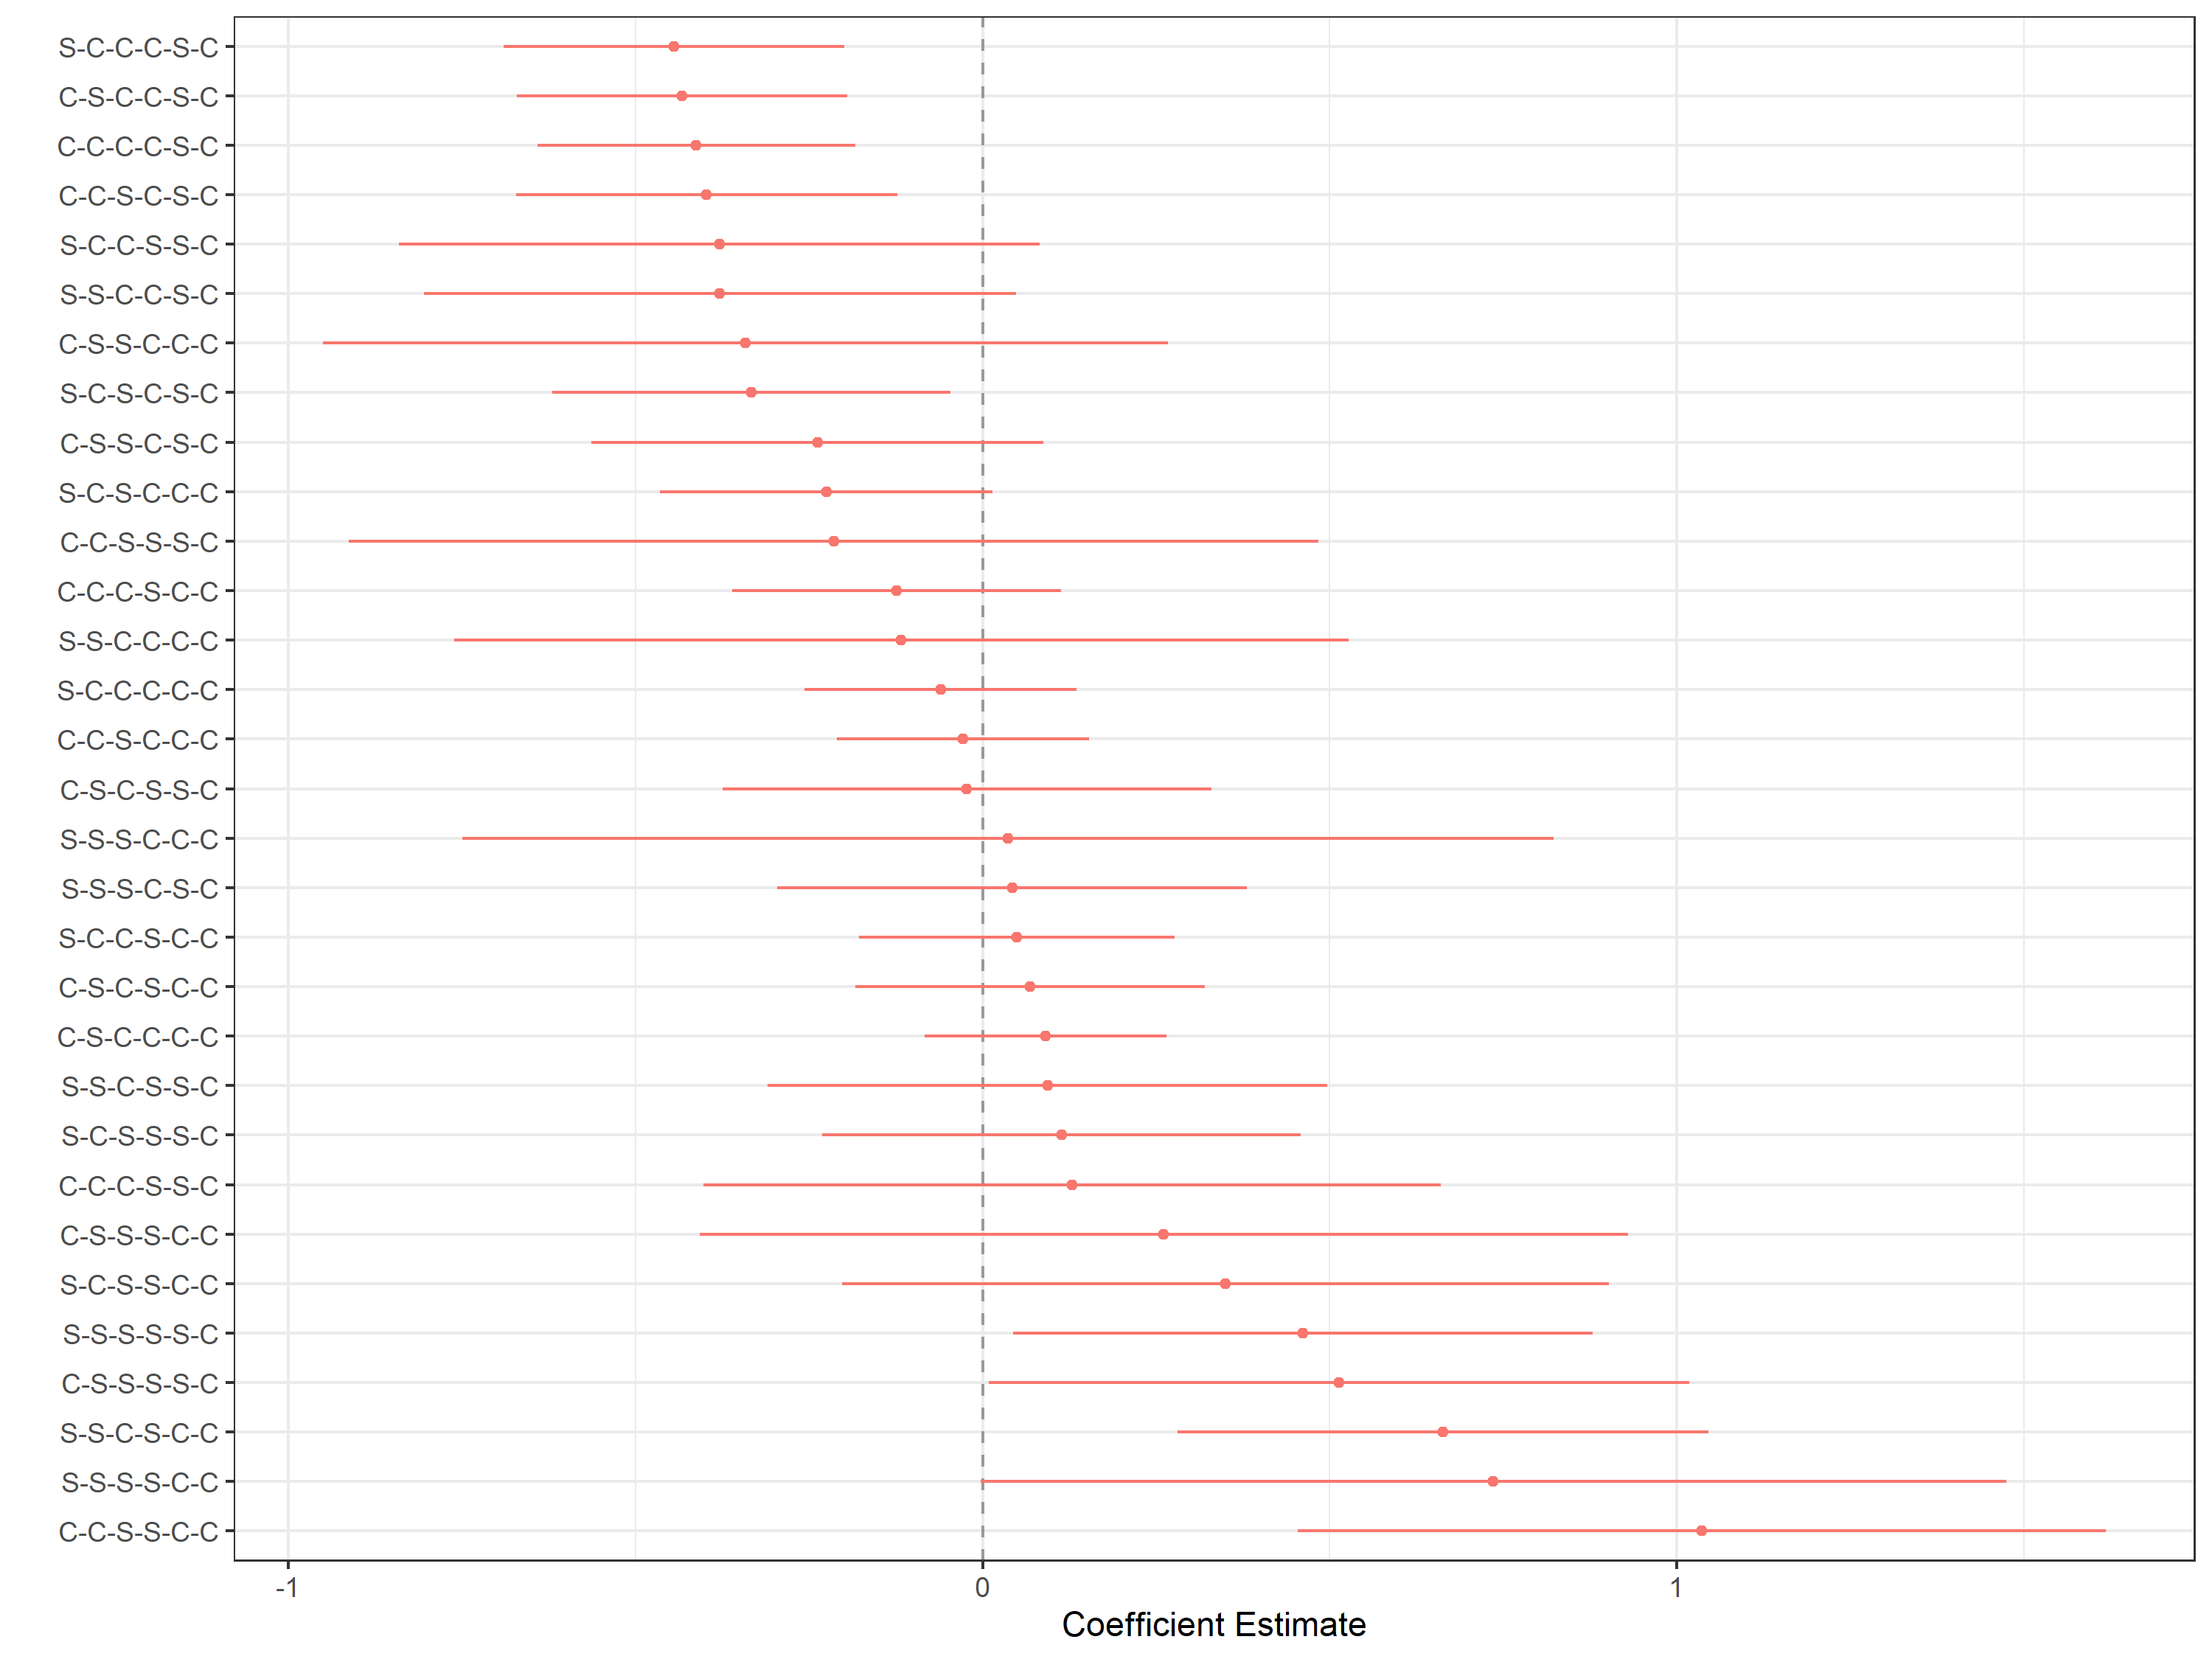
\includegraphics[width=0.90\textwidth]{figures/corn_var_plot}
  \caption{Response of the standard deviation of corn yields to rotation sequences.}
  \label{fig:corn_var_plot}
  \floatfoot{\footnotesize Notes: Point estimates and 95\% confidence intervals
  from stage-2 FGLS variance regression. Reference: corn monoculture. Two-way
  clustering at county and year level.}
\end{figure}

Figure~\ref{fig:corn_jp_plot} summarizes the joint mean-variance results in a single scatter plot.

Table~\ref{tab:corn_jp_moments} (column 2) extends the mean-variance results to the third moment, reporting the effect of each rotation sequence on the standardized conditional skewness of corn yields, estimated as a third-stage regression of the cubed first-stage residual on the same specification (following \citet{antle1983}). The sign convention is the reverse of the variance stage: a \emph{positive} skewness coefficient indicates that a sequence shifts probability mass toward the right tail relative to corn monoculture, thinning the left tail and \emph{reducing} downside risk, whereas a negative coefficient signals heavier left-tail exposure. This margin maps most directly onto insurance loss cost, since indemnities are paid on low-yield realizations rather than on variance per se; a sequence can lower variance while leaving, or worsening, the probability of a bad harvest.

The estimated skewness effects do not reproduce the downside-risk buffering that the experimental diversification literature would lead one to expect. The point estimates are predominantly negative, and every coefficient that is statistically distinguishable from zero is negative: sequences such as C-C-C-S-S-C ($-0.40$), S-S-C-C-C-C ($-0.36$), and C-S-C-S-C-C ($-0.34$) carry the largest significant negative loadings, while no sequence enters with a significantly \emph{positive} skewness coefficient. Read against the sign convention above, this means the rotation sequences that move corn's third moment at all move it toward \emph{heavier} left tails relative to continuous corn: greater, not lesser, downside exposure. The contrast with \citet{bowles2020} and \citet{difalco2009} is instructive: the resilience benefits documented in long-term diversification experiments and in cross-sectional crop-diversity data do not carry over to temporal rotation as capitalized in these field-scale corn yields. Combined with the mean and variance results, few, if any, sequences clear a three-moment dominance screen over monoculture: higher mean, lower variance, and no increase in downside risk simultaneously. For the paper's central question, this cuts in a consistent direction: it is further evidence that rotation history does not map onto corn yield risk in a clean, monotone way.

\begin{figure}[H]
  \centering
  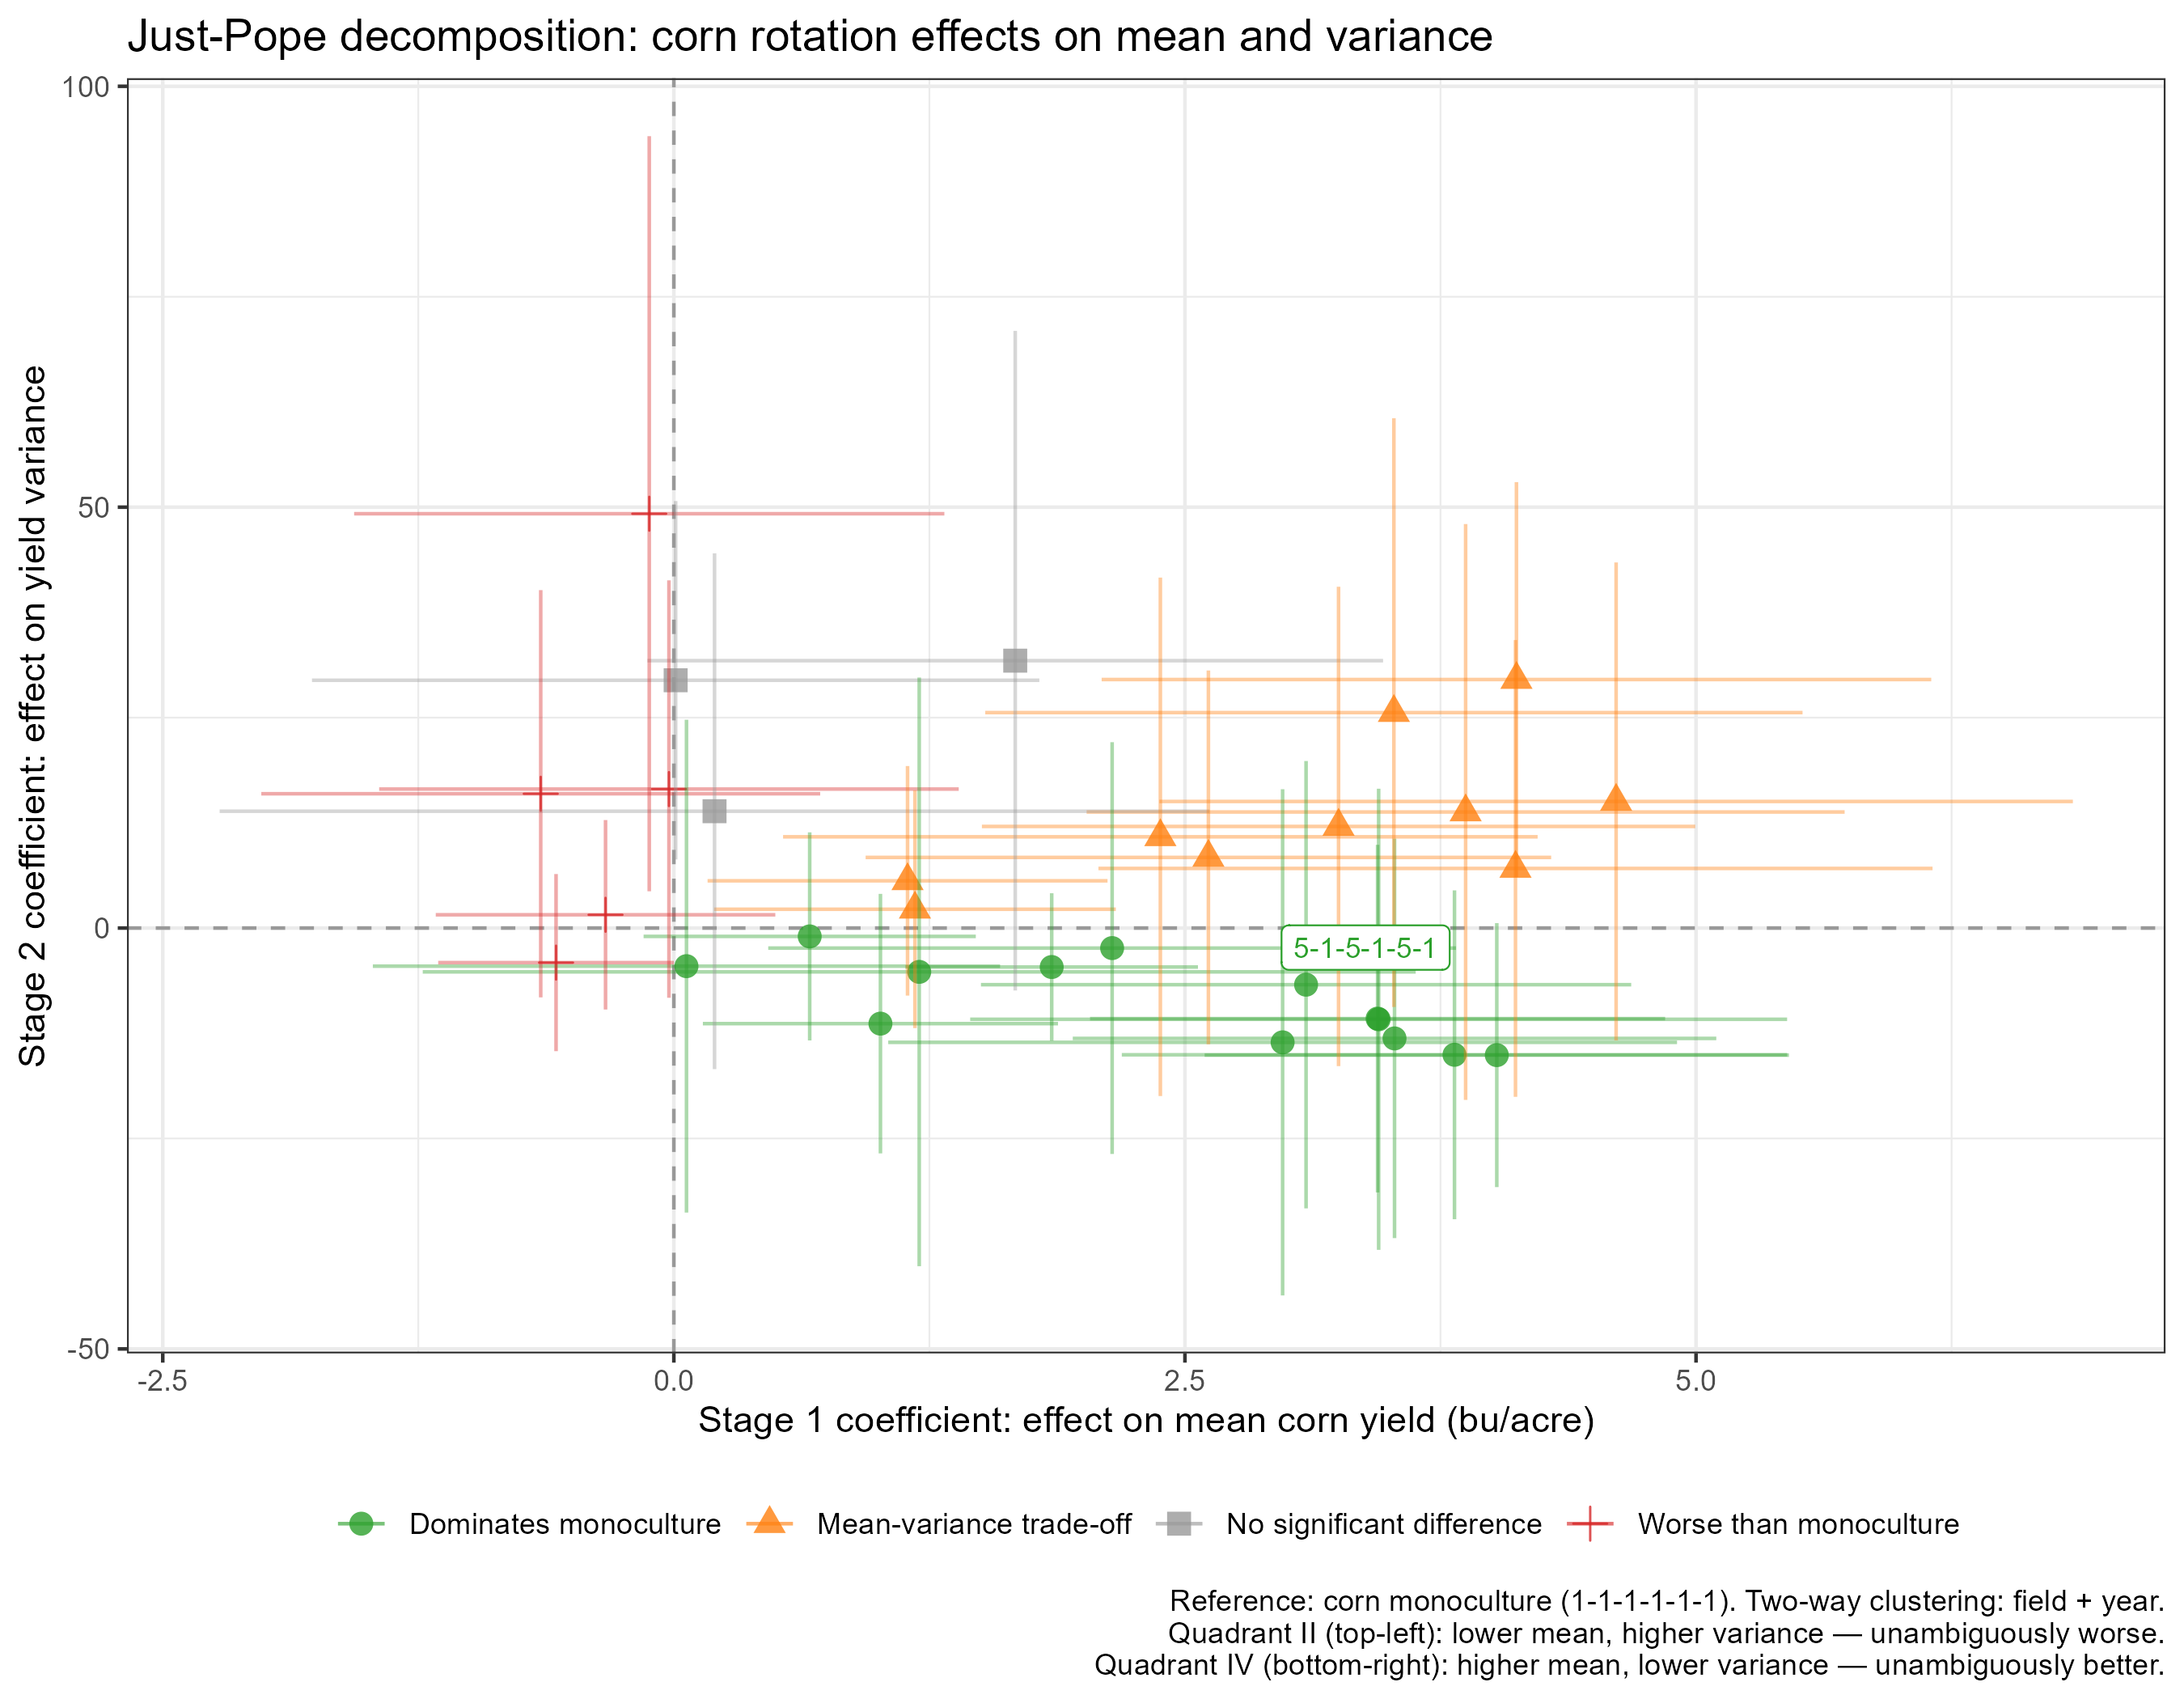
\includegraphics[width=0.85\textwidth]{figures/corn_jp_plot}
  \caption{Just-Pope decomposition: corn rotation effects on mean and variance.}
  \label{fig:corn_jp_plot}
  \floatfoot{\footnotesize Notes: Each point represents one of the 28
  non-monoculture rotation sequences (23 corn-soybeans, 5 corn-soybeans-wheat).
  Horizontal axis: stage-1 coefficient (effect on mean corn yield). Vertical
  axis: stage-2 FGLS coefficient (effect on yield variance). Error bars are 95\%
  confidence intervals. Green (``Dominates monoculture''): higher mean
  \textit{and} lower variance than monoculture. Orange (``Mean-variance
  trade-off''): higher mean, higher variance. Red (``Worse than monoculture''):
  lower mean. Grey (``No significant difference''): not significantly different
  from monoculture.
  }
\end{figure}

\subsection{\label{subsec:lasso_results}LASSO-Selected Rotation Sequences}

Of the 102 candidate corn sequences in the unrestricted sample, 29 survive LASSO selection with a nonzero post-selection coefficient (28.4\% of the sample; Table~\ref{tab:corn_lasso}).

As a robustness check on the selection, we compare the sequences selected by the plug-in-penalty \texttt{rlasso} against a \texttt{cv.glmnet} fit with the same demeaned outcome and design matrix. \texttt{cv.glmnet} selects 28 sequences at the 1-SE lambda against \texttt{rlasso}'s 29, and the two procedures agree on 26 sequences (89.7\% of \texttt{rlasso}'s selections). Agreement is not one-directional: three sequences are selected by \texttt{rlasso} only and two by \texttt{cv.glmnet} only, so each procedure picks up a small number of sequences the other misses rather than one nesting inside the other. None of the five disputed sequences is individually discussed elsewhere in this paper.


\begingroup
\centering
\begin{tabular}{lc}
   \tabularnewline \midrule \midrule
   Dependent Variable: & corn\_yield\\   
   Model:              & (1)\\  
   \midrule
   \emph{Variables}\\
   1-1-1-1-5-1         & 4.502$^{***}$\\   
                       & (0.3549)\\   
   1-1-1-5-1-1         & 2.164$^{***}$\\   
                       & (0.2464)\\   
   1-1-1-5-24-1        & 5.818$^{***}$\\   
                       & (0.6551)\\   
   1-1-1-5-5-1         & 3.921$^{***}$\\   
                       & (0.5005)\\   
   1-1-5-1-1-1         & 0.7593$^{***}$\\   
                       & (0.2786)\\   
   1-1-5-1-5-1         & 4.259$^{***}$\\   
                       & (0.3833)\\   
   1-5-1-1-1-1         & -0.6948$^{***}$\\   
                       & (0.2471)\\   
   1-5-1-1-5-1         & 4.295$^{***}$\\   
                       & (0.3548)\\   
   1-5-1-24-5-1        & 5.834$^{***}$\\   
                       & (1.494)\\   
   1-5-1-5-1-1         & 1.189$^{***}$\\   
                       & (0.3537)\\   
   1-5-1-5-5-1         & 4.582$^{***}$\\   
                       & (0.6346)\\   
   1-5-5-5-5-1         & 4.287$^{***}$\\   
                       & (0.5440)\\   
   24-1-1-5-24-1       & 7.398$^{***}$\\   
                       & (1.383)\\   
   5-1-1-1-1-1         & -1.004$^{***}$\\   
                       & (0.2284)\\   
   5-1-1-1-5-1         & 4.474$^{***}$\\   
                       & (0.3386)\\   
   5-1-1-5-24-1        & 4.185$^{***}$\\   
                       & (0.6791)\\   
   5-1-1-5-5-1         & 3.586$^{***}$\\   
                       & (0.5740)\\   
   5-1-5-1-1-1         & 0.3593\\   
                       & (0.4155)\\   
   5-1-5-1-5-1         & 4.017$^{***}$\\   
                       & (0.3780)\\   
   5-1-5-24-5-1        & 6.173$^{***}$\\   
                       & (0.6343)\\   
   5-1-5-5-1-1         & 0.6851\\   
                       & (0.5349)\\   
   5-1-5-5-5-1         & 4.841$^{***}$\\   
                       & (0.4516)\\   
   5-5-1-1-1-1         & -1.304$^{**}$\\   
                       & (0.6389)\\   
   5-5-1-1-5-1         & 4.579$^{***}$\\   
                       & (0.4919)\\   
   5-5-1-5-1-1         & -0.4512\\   
                       & (0.5500)\\   
   5-5-1-5-5-1         & 5.924$^{***}$\\   
                       & (0.5177)\\   
   5-5-5-1-5-1         & 3.386$^{***}$\\   
                       & (0.4969)\\   
   5-5-5-5-5-1         & 4.745$^{***}$\\   
                       & (0.5480)\\   
   pr\_6               & 0.2115$^{***}$\\   
                       & (0.0201)\\   
   pr\_7               & 0.1022$^{***}$\\   
                       & (0.0146)\\   
   pr\_8               & 0.0393$^{***}$\\   
                       & (0.0116)\\   
   I(I(pr\_6\^2))      & -0.0008$^{***}$\\   
                       & ($5.97\times 10^{-5}$)\\    
   I(I(pr\_7\^2))      & -0.0002$^{***}$\\   
                       & ($5.8\times 10^{-5}$)\\    
   I(I(pr\_8\^2))      & -0.0001$^{***}$\\   
                       & ($3.42\times 10^{-5}$)\\    
   cGDD\_6m            & 0.6102$^{***}$\\   
                       & (0.1058)\\   
   cGDD\_7m            & -0.0507\\   
                       & (0.0887)\\   
   cGDD\_8m            & 0.4222$^{***}$\\   
                       & (0.0556)\\   
   EDD\_6              & -19.65$^{***}$\\   
                       & (2.722)\\   
   EDD\_7              & 0.7623\\   
                       & (2.429)\\   
   EDD\_8              & -12.00$^{***}$\\   
                       & (1.710)\\   
   vpd\_6              & 54.03$^{***}$\\   
                       & (6.985)\\   
   vpd\_7              & -19.23$^{***}$\\   
                       & (4.511)\\   
   vpd\_8              & 9.816$^{***}$\\   
                       & (3.431)\\   
   soil\_6             & -0.0798$^{***}$\\   
                       & (0.0222)\\   
   soil\_7             & -0.0268\\   
                       & (0.0219)\\   
   soil\_8             & 0.0089\\   
                       & (0.0143)\\   
   \midrule
   \emph{Fixed-effects}\\
   tile\_field\_ID     & Yes\\  
   year                & Yes\\  
   \midrule
   \emph{Fit statistics}\\
   Observations        & 1,640,572\\  
   R$^2$               & 0.83832\\  
   Within R$^2$        & 0.14358\\  
   \midrule \midrule
   \multicolumn{2}{l}{\emph{Clustered (COUNTY\_FIPS) standard-errors in parentheses}}\\
   \multicolumn{2}{l}{\emph{Signif. Codes: ***: 0.01, **: 0.05, *: 0.1}}\\
\end{tabular}
\par\endgroup



\begin{quote}
\small
Notes: Dependent variable is QDANN corn yield. Coefficients are from an unpenalized fixed-effects refit restricted to the 29 sequences with nonzero LASSO coefficients (post-selection OLS; see Section~\ref{subsec:stage_1}), not the LASSO coefficients themselves. Reference category: continuous corn. Sample and control vector as in Table~\ref{tab:corn_rot}, except the sequence set is the unrestricted 102-sequence candidate pool rather than the 29-sequence, 99\%-frequency-restricted sample, so the sample size differs from Table~\ref{tab:corn_rot}. Field (tile\_field\_ID) and year fixed effects included; standard errors clustered at county (COUNTY\_FIPS).
\end{quote}

The selected corn sequences show one clear pattern. Coefficients are consistently large and positive when the most recent rotation year (six years back through the current year) includes a soybean planting close to the current year, and consistently small, negative, or insignificant when the only soybean year in the window is five years distant and the intervening years are continuous corn. For example, a single distant soybean year followed by four years of continuous corn (S-C-C-C-C-C and C-S-C-C-C-C) carries significant \emph{negative} coefficients, while sequences with soybean in the year immediately preceding the current corn crop are uniformly positive and significant. This is the same recency pattern documented by the Z-vector's $\text{late\_soy}$ coefficient below, recovered here by a purely data-driven selection procedure rather than an assumed functional form, which is a useful cross-validation of that result. Of the 29 selected corn sequences, four (C-C-S-S-C-C, S-C-S-C-C-C, S-C-S-S-C-C, and S-S-C-S-C-C) are not statistically significant in the post-selection refit, indicating that LASSO selection and conventional significance are not the same criterion; a sequence can survive the penalty and still fail to clear significance once shrinkage is removed.

\subsection{Parsimonious Z-Vector Model}


\begin{table}[htbp]
   \caption{\label{tab:zvector} Effect of rotation patterns on yields}
   \bigskip
   \centering
   \begin{tabular}{lcc}
      \toprule
                                      & corn\_yield             & resid\_sq\_z\\
                                      & Corn mean               & Corn variance \\
                                      & (1)                     & (2)\\
      \midrule
      Latest soy rotation             & 0.4470$^{***}$ (0.0612) & -0.5826 (0.9477)\\
      Soy gap                         & 0.6928$^{***}$ (0.1509) & -3.748$^{*}$ (2.042)\\
      Number of consecutive soy years & 1.210$^{**}$ (0.4396)   & 6.878 (3.971)\\
       \\
      Observations                    & 1,785,861               & 1,785,861\\
      R$^2$                           & 0.84288                 & 0.29040\\
      Within R$^2$                    & 0.15022                 & 0.01383\\
      Controls                        & Yes                     & Yes\\
      tile\_field\_ID FE              & $\checkmark$            & $\checkmark$\\
      Year FE                         & $\checkmark$            & $\checkmark$\\
      \bottomrule
   \end{tabular}
\end{table}

\begin{quote}
\small
Notes: Columns (1)-(2) report corn yield mean and variance effects, discussed below. Columns (1) and (2) are stage-1 and stage-2 (OLS on squared residuals) coefficients, respectively. Controls include monthly precipitation (quadratic), GDD, EDD, VPD, and soil moisture for June-August. Field (tile\_field\_ID) and year fixed effects are included. Column (1) standard errors are two-way clustered at the county and year level. Because the column (2) dependent variable is a generated regressor (the squared stage-1 residual), its standard errors are from a $B=999$ field-level pairs cluster bootstrap wrapping both stages (Section~\ref{subsec:bootstrap}); the analytic two-way clustered counterparts are $0.90$, $1.96$, and $3.94$. $^{***}p<0.01$, $^{**}p<0.05$, $^{*}p<0.10$.
\end{quote}
Table~\ref{tab:zvector} reports the parsimonious parameterization of rotation effects in terms of three structural features of soybean placement within the six-year corn rotation window: recency, spacing, and consecutiveness.

For corn yields, all three features carry positive mean effects. The most recent soybean placement variable ($\text{late\_soy}$) has a mean effect of 0.447 ($p<0.01$) and the soybean-gap variable has a larger effect of 0.693 ($p<0.01$): both a more recent soybean harvest and wider spacing between soybean years raise mean corn yields. The consecutive-soybean-years variable carries a positive mean effect of 1.210 ($p<0.05$). Because the soybean-gap feature now also absorbs the overall soybean-frequency signal previously carried by the (dropped) count feature, its coefficient should be read as the combined effect of spacing and frequency rather than spacing holding frequency fixed.

The variance equation is stronger under the bootstrap than under analytic standard errors. All three features enter with signs that match the mean results: wider soybean spacing ($\text{soy\_gap}$, $-3.75$) and a more recent soybean placement ($\text{late\_soy}$, $-0.58$) are associated with \emph{lower} corn yield variance. In contrast, consecutive soybean years raise it ($\text{soy\_cons}$, $+6.88$). Because column (2) has a generated-regressor dependent variable, the inference of record is the $B=999$ field-level pairs cluster bootstrap that wraps both stages (Section~\ref{subsec:bootstrap}), the same design used for the sequence-dummy variance stage in Table~\ref{tab:corn_jp_moments}. Under that bootstrap, all three coefficients are significant: the soybean gap and consecutive-soybean years at the 1\% level, recency at 5\%. Analytic two-way clustered standard errors, by contrast, leave the gap effect marginal ($p<0.10$) and the other two insignificant. The bootstrap intervals are several times tighter than the analytic ones, and the gap persists whether the analytic standard errors cluster at the county or field level, so it reflects the bootstrap's propagation of first-stage estimation error rather than the choice of clustering dimension. Field resampling captures the within-field serial correlation that dominates the panel but not any residual cross-field correlation within counties, so we read wider soybean spacing as a robust variance-reducing feature and treat recency and consecutiveness as directionally consistent.

\subsection{\label{subsec:rot_score_res}Rotation Score}

\begin{figure}[H]
  \centering
  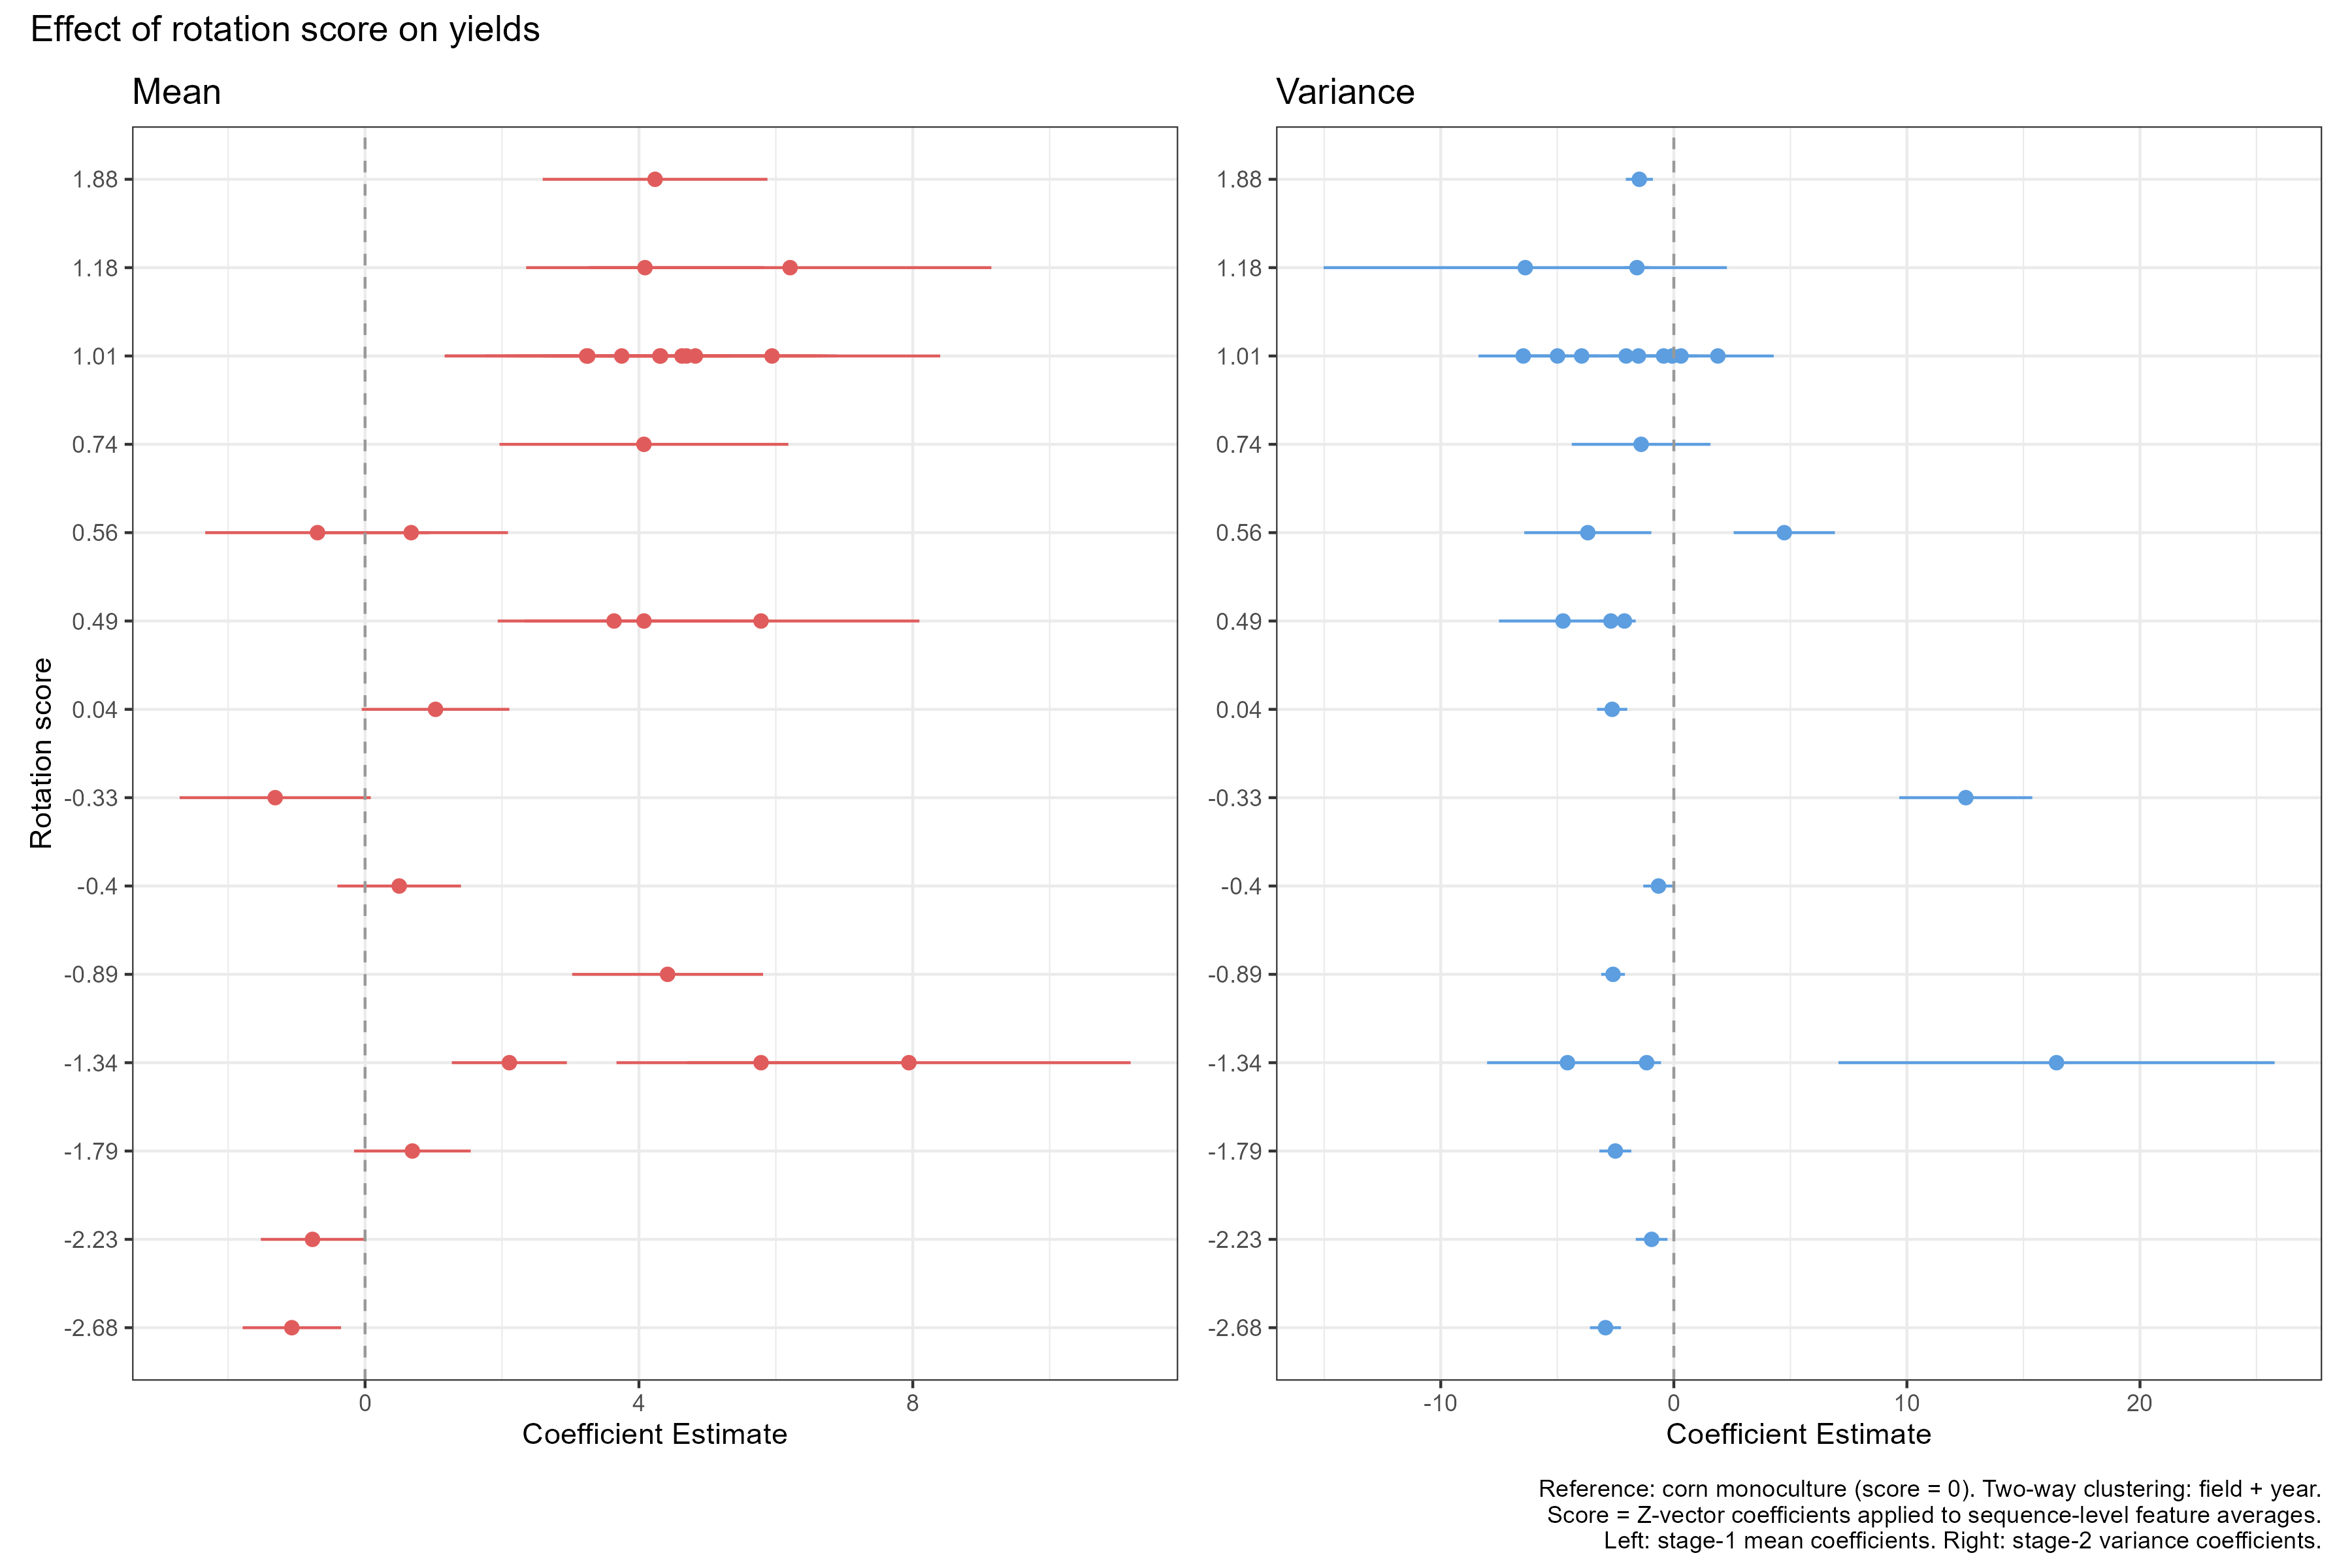
\includegraphics[width=\textwidth]{figures/score_yield}
  \caption{Effect of rotation score on corn yields.}
  \label{fig:score_yield}
  \floatfoot{\footnotesize Notes: Rotation score computed by applying the
  Z-vector coefficients from Table~\ref{tab:zvector} to sequence-level feature
  averages, per equation~\eqref{eq:score}. Left panel: stage-1 coefficient on
  mean corn yield. Right panel: stage-2 coefficient on conditional yield
  variance. Horizontal bars are 95\% confidence intervals. Reference: corn
  monoculture (score $= 0$). Two-way clustering at county and year level.
  Source: QDANN yield estimates, \citet{Ma2024}; CDL rotation histories,
  USDA-NASS.}
\end{figure}

Figure~\ref{fig:score_yield} reports predicted corn yields as a function of the rotation score, computed over the 28-sequence corn-soybeans-wheat sample using the three-feature Z-vector coefficients. A direct summary of the scoring pipeline's output (\texttt{score\_plot\_df}, 28 sequences) shows the score running from $-2.68$ to $+1.88$ relative to corn monoculture (normalized to zero), with mean $0.16$ and median $0.56$; the distribution is left-skewed, the mean sitting below the median as a small number of poorly-scoring sequences pull the lower tail down. The 28 sequences map onto 14 distinct score values, with several sequences sharing an identical score, and the perfect alternating rotation (S-C-S-C-S-C) scores $+0.49$ (mean-yield coefficient $3.64$, $p<0.001$). The score-yield relationship is positive overall but noisy in the middle of the distribution rather than cleanly monotone; variance effects show no clean monotone relationship with score across the distribution.

\subsection{\label{subsec:vpd_effects}Weather Effects: Vapor Pressure Deficit and Drought}


\begin{table}[H]
   \caption{\label{tab:corn_rot_vpd} Effect of weather and rotation sequences on corn yields}
   \bigskip
   \centering
   \begin{tabular}{lc}
      \toprule
                                      & corn\_yield\\   
                                      & (1)\\  
      \midrule 
      C-C-C-C-S-C                     & 277.7$^{***}$\\   
                                      & (22.12)\\   
      C-C-C-S-C-C                     & 131.5$^{***}$\\   
                                      & (15.30)\\   
      C-C-C-S-S-C                     & 228.9$^{***}$\\   
                                      & (32.46)\\   
      C-C-C-S-W-C                     & 384.3$^{***}$\\   
                                      & (38.80)\\   
      C-C-S-C-C-C                     & 43.95$^{**}$\\   
                                      & (17.40)\\   
      C-C-S-C-S-C                     & 257.4$^{***}$\\   
                                      & (23.81)\\   
      C-C-S-S-C-C                     & -4.510\\   
                                      & (39.44)\\   
      C-C-S-S-S-C                     & 200.9$^{***}$\\   
                                      & (36.06)\\   
      C-C-S-W-C-C                     & 108.2$^{***}$\\   
                                      & (38.37)\\   
      C-S-C-C-C-C                     & -47.56$^{***}$\\   
                                      & (15.51)\\   
      C-S-C-C-S-C                     & 255.0$^{***}$\\   
                                      & (22.50)\\   
      C-S-C-S-C-C                     & 65.09$^{***}$\\   
                                      & (21.98)\\   
      C-S-C-S-S-C                     & 306.0$^{***}$\\   
                                      & (39.33)\\   
      C-S-C-S-W-C                     & 180.2$^{***}$\\   
                                      & (33.56)\\   
      C-S-S-C-C-C                     & 30.26\\   
                                      & (36.88)\\   
      C-S-S-C-S-C                     & 150.7$^{***}$\\   
                                      & (35.26)\\   
      C-S-S-S-C-C                     & 55.87\\   
                                      & (51.37)\\   
      C-S-S-S-S-C                     & 270.2$^{***}$\\   
                                      & (32.86)\\   
      C-S-W-C-C-C                     & -9.819\\   
                                      & (48.84)\\   
      C-S-W-C-S-C                     & 210.8$^{***}$\\   
                                      & (33.88)\\   
      S-C-C-C-C-C                     & -66.98$^{***}$\\   
                                      & (14.33)\\   
      S-C-C-C-S-C                     & 270.4$^{***}$\\   
                                      & (21.06)\\   
      S-C-C-S-C-C                     & 96.94$^{***}$\\   
                                      & (20.56)\\   
      S-C-C-S-S-C                     & 222.4$^{***}$\\   
                                      & (33.76)\\   
      S-C-C-S-W-C                     & 268.7$^{***}$\\   
                                      & (41.97)\\   
      S-C-S-C-C-C                     & 16.17\\   
                                      & (26.10)\\   
      S-C-S-C-S-C                     & 240.3$^{***}$\\   
                                      & (23.51)\\   
      S-C-S-C-W-C                     & 194.9$^{***}$\\   
                                      & (56.08)\\   
      S-C-S-S-C-C                     & 33.92\\   
                                      & (33.77)\\   
      S-C-S-S-S-C                     & 298.3$^{***}$\\   
                                      & (28.21)\\   
      S-C-S-W-C-C                     & 80.31$^{*}$\\   
                                      & (41.33)\\   
      S-C-S-W-S-C                     & 366.3$^{***}$\\   
                                      & (38.62)\\   
      S-C-W-C-S-C                     & 119.5$^{*}$\\   
                                      & (60.66)\\   
      S-S-C-C-C-C                     & -81.67$^{**}$\\   
                                      & (39.45)\\   
      S-S-C-C-S-C                     & 272.6$^{***}$\\   
                                      & (31.57)\\   
      S-S-C-S-C-C                     & -24.08\\   
                                      & (34.37)\\   
      S-S-C-S-S-C                     & 371.6$^{***}$\\   
                                      & (31.44)\\   
      S-S-S-C-C-C                     & 12.65\\   
                                      & (43.12)\\   
      S-S-S-C-S-C                     & 205.5$^{***}$\\   
                                      & (31.18)\\   
      S-S-S-S-C-C                     & 134.2$^{**}$\\   
                                      & (53.53)\\   
      S-S-S-S-S-C                     & 289.0$^{***}$\\   
                                      & (34.68)\\   
      S-W-C-C-S-C                     & 234.1$^{***}$\\   
                                      & (39.10)\\   
      S-W-C-S-C-C                     & 0.8649\\   
                                      & (45.91)\\   
      S-W-C-S-S-C                     & 278.1$^{***}$\\   
                                      & (60.27)\\   
      S-W-C-S-W-C                     & 261.5$^{***}$\\   
                                      & (57.85)\\   
      S-W-S-C-S-C                     & 183.5$^{***}$\\   
                                      & (55.72)\\   
      W-C-C-C-C-C                     & 129.9$^{*}$\\   
                                      & (67.68)\\   
      W-C-S-C-S-C                     & 198.4$^{***}$\\   
                                      & (36.50)\\   
      Somewhat dry season             & -95.32$^{***}$\\   
                                      & (34.73)\\   
      Dry season                      & -139.7$^{***}$\\   
                                      & (53.19)\\   
       \\
      Observations                    & 1,741,050\\  
      R$^2$                           & 0.84021\\  
      Within R$^2$                    & 0.14688\\  
       \\
      tile\_field\_ID fixed effects   & $\checkmark$\\   
      year fixed effects              & $\checkmark$\\   
      \bottomrule
   \end{tabular}
\end{table}



\begin{quote}
\small
Notes: Dependent variable is QDANN corn yield in bushels per acre. Rotation
sequences enter as indicators relative to corn monoculture (C-C-C-C-C-C).
\emph{Somewhat dry season} and \emph{Dry season} are July vapor pressure deficit
(VPD) bins, defined as 1.9-2.1 kPa and $>$2.1 kPa, respectively, with normal
($<$1.9 kPa) as the omitted reference. Continuous monthly VPD was dropped for
collinearity with the July bins and the rest of the monthly weather block, which
also includes precipitation (quadratic), GDD, EDD, and soil moisture for
June-August. Field
(\texttt{tile\_field\_ID}) and year fixed effects included; standard errors
two-way clustered at county and year, in parentheses. $^{***}p<0.01$,
$^{**}p<0.05$, $^{*}p<0.10$.
\end{quote}

Table~\ref{tab:corn_rot_vpd} augments the sequence-mean specification with explicit growing-season weather terms, allowing rotation and drought effects to be read from a single model. July drought enters through two indicator bins defined from the July VPD maximum (\emph{somewhat dry}, 1.9-2.1 kPa; \emph{dry}, $>$2.1 kPa; both relative to a normal July) rather than as a continuous VPD term, which was too collinear with the rest of the monthly weather block to be separately identified. The drought bins are negative and increase in magnitude with severity: a somewhat dry July is associated with a 0.92 bushels-per-acre lower corn yield and a dry July with 1.64 bushels per acre. However, neither bin is individually statistically significant.

The rotation-sequence coefficients retain the ordering documented in Section~\ref{subsec:seq_effects}: sequences combining a recent soybean harvest with winter wheat (for example W-C-C-S-W-C and C-S-C-W-S-C) sit at the top of the table, while continuous-corn-adjacent sequences (C-S-C-C-C-C, S-C-C-C-C-C, S-S-C-C-C-C) carry negative and significant coefficients. That this ordering survives the inclusion of explicit weather controls indicates the rotation effects are not merely proxying for cross-field differences in drought exposure. For insurance rating, the joint result is that drought risk and rotation history enter corn yields through distinct channels: a rotation-conditioned rate would need to price the sequence effect on top of, rather than as a substitute for, the weather-driven component of yield risk.

\section{\label{sec:conclusions}Discussion and Conclusions}

\subsection{\label{susec:summary}Summary of Findings}

This paper uses a large satellite-based field-level panel of Illinois corn yields from 2008 to 2022, with rotation histories built from Cropland Data Layer records back to 2002, to estimate how six-year crop rotation sequences affect both the mean and variance of corn yields. Our main findings are three.

First, the effect of crop rotation on corn yields depends critically on the timing and spacing of soybean placements within the six-year rotation window. A recent soybean harvest raises corn yields by approximately 0.447 ($p<0.01$), and a larger gap between soybean years raises corn yields by approximately 0.693 ($p<0.01$); consecutive soybean years carry a positive mean effect of 1.210 ($p<0.05$). Because the gap feature also absorbs the overall soybean-frequency signal (the soybean-count feature is dropped for collinearity), its coefficient reflects spacing and frequency jointly. A data-driven LASSO selection over the unrestricted candidate sequence space recovers the same recency-and-spacing ordering without imposing it.

Second, the variance effects are estimated less precisely than the mean effects but point in the same direction. Wider soybean spacing is associated with lower corn yield variance, and under the field-level pairs cluster bootstrap appropriate to this generated-regressor stage (Section~\ref{subsec:bootstrap}) the spacing effect is significant at the 1\% level, with recency and consecutiveness also entering significantly and with the signs of the mean effects. The analytic two-way-clustered standard errors are considerably wider and leave the spacing effect only marginal, so the weight one puts on the variance channel depends on the inference adopted; we treat spacing as a robust risk-reducing feature and the other two as directionally consistent. The third-moment results, by contrast, run against the mean and variance findings: the sequences with a detectable skewness effect all shift probability mass toward the left tail, so few sequences achieve joint dominance across all three moments.

Third, we develop a rotation score, constructed from the three structural sequence features, that maps the observed six-year rotation sequences onto 14 distinct scalar values across 28 sequences, ranging from $-2.68$ to $+1.88$ relative to corn monoculture, suitable as a rating input.

\subsection{\label{subsec:implications}Implications for Crop Insurance Rating}

Our findings have direct implications for how federal crop insurance could incorporate rotation information. The rotation score provides a tractable rating instrument: the existing APH framework could implement a premium discount for fields with high rotation scores by conditioning the base premium rate on the CDL-derived score, which is publicly available at the field level at no marginal cost to the insurer. The score's actuarial value rests primarily on its mean-yield content, which is precisely estimated; the corresponding effects on yield variance are directionally consistent (wider soybean spacing is associated with lower variance) and significant under the variance-stage bootstrap, though wider under analytic standard errors, so we treat a variance-based adjustment as plausible but secondary here. Translating the mean-yield effects into expected-indemnity dollar terms under Revenue Protection is a natural next step, but we have not done so here.

One challenge complicates straightforward implementation: the transition penalty we document implies that the APH would temporarily fall for fields moving from monoculture toward a corn-soy rotation, reducing the insurance guarantee precisely when farmers are bearing the costs of practice change, consistent with \citet{Connor2022}. A rotation-conditioned rate should handle this asymmetry explicitly, for example by using the score only after a minimum number of years in the target rotation.

\subsection{\label{subsec:limitations}Limitations and Future Work}

Our analysis has several limitations. First, the yield data come from a satellite-based estimator (QDANN) with a meaningful field-level error rate, and, following \citet{Benami2026}, this measurement error need not be classical. If QDANN's prediction error is uncorrelated with rotation history, it behaves as classical measurement error. It attenuates our rotation effect estimates toward zero, suggesting the true agronomic rotation premium may be larger than what we document. If, however, QDANN's accuracy varies systematically with field characteristics that are themselves correlated with rotation choice, for example, if prediction error differs with field heterogeneity, management intensity, or the confidence of the underlying CDL crop classification, the resulting non-classical measurement error could bias our estimates in either direction, not only toward zero. We do not have the tools to rule out this possibility here and flag it as a first-order concern for future work using EO-derived yield products for rotation-effect estimation.

Second, our identification strategy relies on within-field variation in rotation sequences over time. Field fixed effects absorb any time-invariant field characteristics that could jointly drive rotation choice and yield. Identification then comes only from fields that change rotation patterns during the panel, and time-varying unobservables correlated with those switches remain a threat.

Third, our analysis covers corn rotations involving soybean and winter wheat in Illinois. Winter wheat enters through a minority of sequences and on thin support, so read its estimates as suggestive. Perennial forages such as alfalfa, together with winter-wheat/soybean double crops, are too rare (each well under one percent of field-years) to survive the 99\%-frequency restriction used for the main sequence-dummy and Z-vector results, and are absent from those tables entirely; the LASSO analysis in Section~\ref{subsec:lasso_results}, run over a substantially larger unrestricted candidate set, does not recover any alfalfa-containing sequence for corn either, so we leave a fuller treatment of perennial forage rotations to settings where alfalfa is more common. Generalizability to other Corn Belt states and to different climate and soil regimes is an open question. Finally, rotation decisions respond endogenously to prices and the proximity of grain market infrastructure such as ethanol refineries \citep{Pates2025,cheu2025}. A full welfare analysis of rotation-conditioned rates would require modeling the joint distribution of rotation choice and yield outcomes under the counterfactual rate schedule, which we leave for future work.

\section{\label{sec:conclusion}Conclusion}

This paper shows that crop rotation history carries information about both the mean and the variance of corn yields that APH-based crop insurance rating currently does not capture. Using a satellite-based, field-level panel of Illinois corn fields, we find that the timing and spacing of soybean placement within a six-year rotation window is what predicts yield outcomes. A recent soybean harvest and a wider gap between soybean years are each associated with significantly higher mean corn yields, and with lower yield variance; under the bootstrap inference used for the variance stage, the spacing effect on variance is significant at the 1\% level, though its analytic standard errors are wider, so we still emphasize the mean channel for rating.

To make this evidence usable for rating purposes, we construct a rotation score from three structural features of the rotation sequence-the recency of the last soybean harvest, whether soybean years were consecutive, and the minimum gap between soybean harvests-that collapses the observed six-year rotation sequences into a compact, field-computable scalar. Because it is built entirely from Cropland Data Layer histories that USDA already maintains, the score could in principle be attached to any insured field at no additional data cost. A companion paper asks whether the Rotational Complexity Index, the field-scale complexity summary most widely used in the literature, and cross-field spatial spillovers, offer a comparably useful alternative, and finds that they do not.

Two qualifications bound how far these findings can be pushed toward an actual rating change. First, we document effects in bushels per acre and in variance units, not in premium dollars: converting these magnitudes into a rate adjustment, and checking that adjustment against the cross-subsidization concerns raised by \citet{Ramaswami1993} and \citet{Babcock1996}, is necessary before any of this could inform an actual RMA rate filing. Second, our identification comes from a single state and a sample dominated by corn-soybean rotations, with only five winter-wheat sequences entering on thin support; whether the same timing-and-spacing pattern holds more broadly for rotations built around a third crop, for cover crops, or for other Corn Belt geographies is largely untested here. Two extensions follow directly from these gaps and from the analysis above: an explicit premium simulation that maps the rotation score onto a candidate rate adjustment, and an out-of-state replication using the same field-level pipeline. A third, narrower extension-modeling how the APH transition-year penalty documented in Section~\ref{subsec:implications} evolves over the first several years after a field switches into rotation-would directly inform whether a rotation-conditioned rate needs a separate adoption-year adjustment or can rely on the steady-state score alone.

\newpage
\bibliography{bibliography.bib}

\newpage
\ Appendix

\section*{Tables}


\begin{table}[H]
   \caption{\label{tab:corn_jp_moments} Stage 2/3 — Corn yield conditional variance (FGLS) and skewness}
   \bigskip
   \centering
   \begin{tabular}{lcc}
      \toprule
                                      & resid\_sq            & resid\_cube\_std\\    
                                      & Variance             & Skewness (standardized) \\   
                                      & (1)                  & (2)\\  
      \midrule 
      C-C-C-C-S-C                     & -2.608$^{*}$ (1.561) & -0.0761$^{*}$ (0.0442)\\   
      C-C-C-S-C-C                     & -1.166 (1.888)       & -0.1086$^{*}$ (0.0556)\\   
      C-C-C-S-S-C                     & -3.954 (6.955)       & -0.4022$^{*}$ (0.2152)\\   
      C-C-C-S-W-C                     & -4.563 (7.625)       & -0.0806 (0.2647)\\   
      C-C-S-C-C-C                     & -2.510 (1.960)       & 0.0460 (0.0550)\\   
      C-C-S-C-S-C                     & -2.699$^{*}$ (1.543) & -0.0188 (0.0423)\\   
      C-S-C-C-C-C                     & -0.9526 (1.995)      & 0.0669 (0.0680)\\   
      C-S-C-C-S-C                     & -1.582 (1.604)       & 0.0362 (0.0458)\\   
      C-S-C-S-C-C                     & -2.645 (1.800)       & -0.3407$^{***}$ (0.0484)\\   
      C-S-C-S-S-C                     & -0.4388 (2.100)      & -0.2035$^{***}$ (0.0564)\\   
      C-S-C-W-S-C                     & -6.375 (16.24)       & 0.3349 (0.3274)\\   
      C-S-S-S-S-C                     & 1.889 (7.323)        & -0.0663 (0.1385)\\   
      S-C-C-C-C-C                     & -2.932 (1.920)       & -0.0219 (0.0458)\\   
      S-C-C-C-S-C                     & -1.481 (1.712)       & 0.0683 (0.0480)\\   
      S-C-C-S-S-C                     & -4.991 (4.073)       & -0.3224$^{**}$ (0.1262)\\   
      S-C-C-S-W-C                     & -1.404 (9.155)       & -0.1392 (0.2262)\\   
      S-C-S-C-C-C                     & -0.6575 (1.899)      & 0.0018 (0.0525)\\   
      S-C-S-C-S-C                     & -2.120 (1.449)       & -0.0213 (0.0396)\\   
      S-C-S-S-C-C                     & 4.738 (5.055)        & -0.2435$^{**}$ (0.1169)\\   
      S-C-S-S-S-C                     & -1.519 (3.024)       & -0.1926$^{*}$ (0.1060)\\   
      S-C-S-W-S-C                     & -4.754 (5.753)       & 0.0146 (0.1780)\\   
      S-S-C-C-C-C                     & 12.53 (9.702)        & -0.3612$^{**}$ (0.1745)\\   
      S-S-C-C-S-C                     & -2.046 (4.119)       & 0.0272 (0.1042)\\   
      S-S-C-S-C-C                     & -3.690 (6.543)       & -0.2505$^{*}$ (0.1310)\\   
      S-S-C-S-S-C                     & 0.3054 (3.665)       & -0.2254$^{***}$ (0.0870)\\   
      S-S-S-C-S-C                     & -0.0708 (3.020)      & -0.1992$^{***}$ (0.0745)\\   
      S-S-S-S-S-C                     & -6.460 (4.635)       & -0.0717 (0.0857)\\   
      W-C-C-S-W-C                     & 16.42 (21.80)        & -0.2389 (0.2466)\\   
       \\
      Observations                    & 1,785,861            & 1,785,861\\  
      R$^2$                           & 0.60737              & 0.08661\\  
      Within R$^2$                    & 0.00403              & 0.00195\\  
       \\
      tile\_field\_ID fixed effects   & $\checkmark$         & $\checkmark$\\   
      year fixed effects              & $\checkmark$         & $\checkmark$\\   
      \bottomrule
   \end{tabular}
\end{table}



\begin{quote}
\small
Notes: Column (1) reports stage-2 estimates of variance equation~\eqref{eq:stage2} (squared first-stage residual); column (2) reports the third-stage standardized-skewness regression (cubed, standardized first-stage residual), by rotation sequence. Reference: corn monoculture. Field (tile\_field\_ID) and year fixed effects included. Reported here rather than in the main text because the conditional-variance and -skewness estimators are secondary to the mean results in this setting; see Section~\ref{subsec:var_effects}. Inference of record for these stages is the three-stage bootstrap of Section~\ref{subsec:bootstrap}.
\end{quote}

\clearpage
\section*{Figures}

\begin{figure}[H]
  \centering
  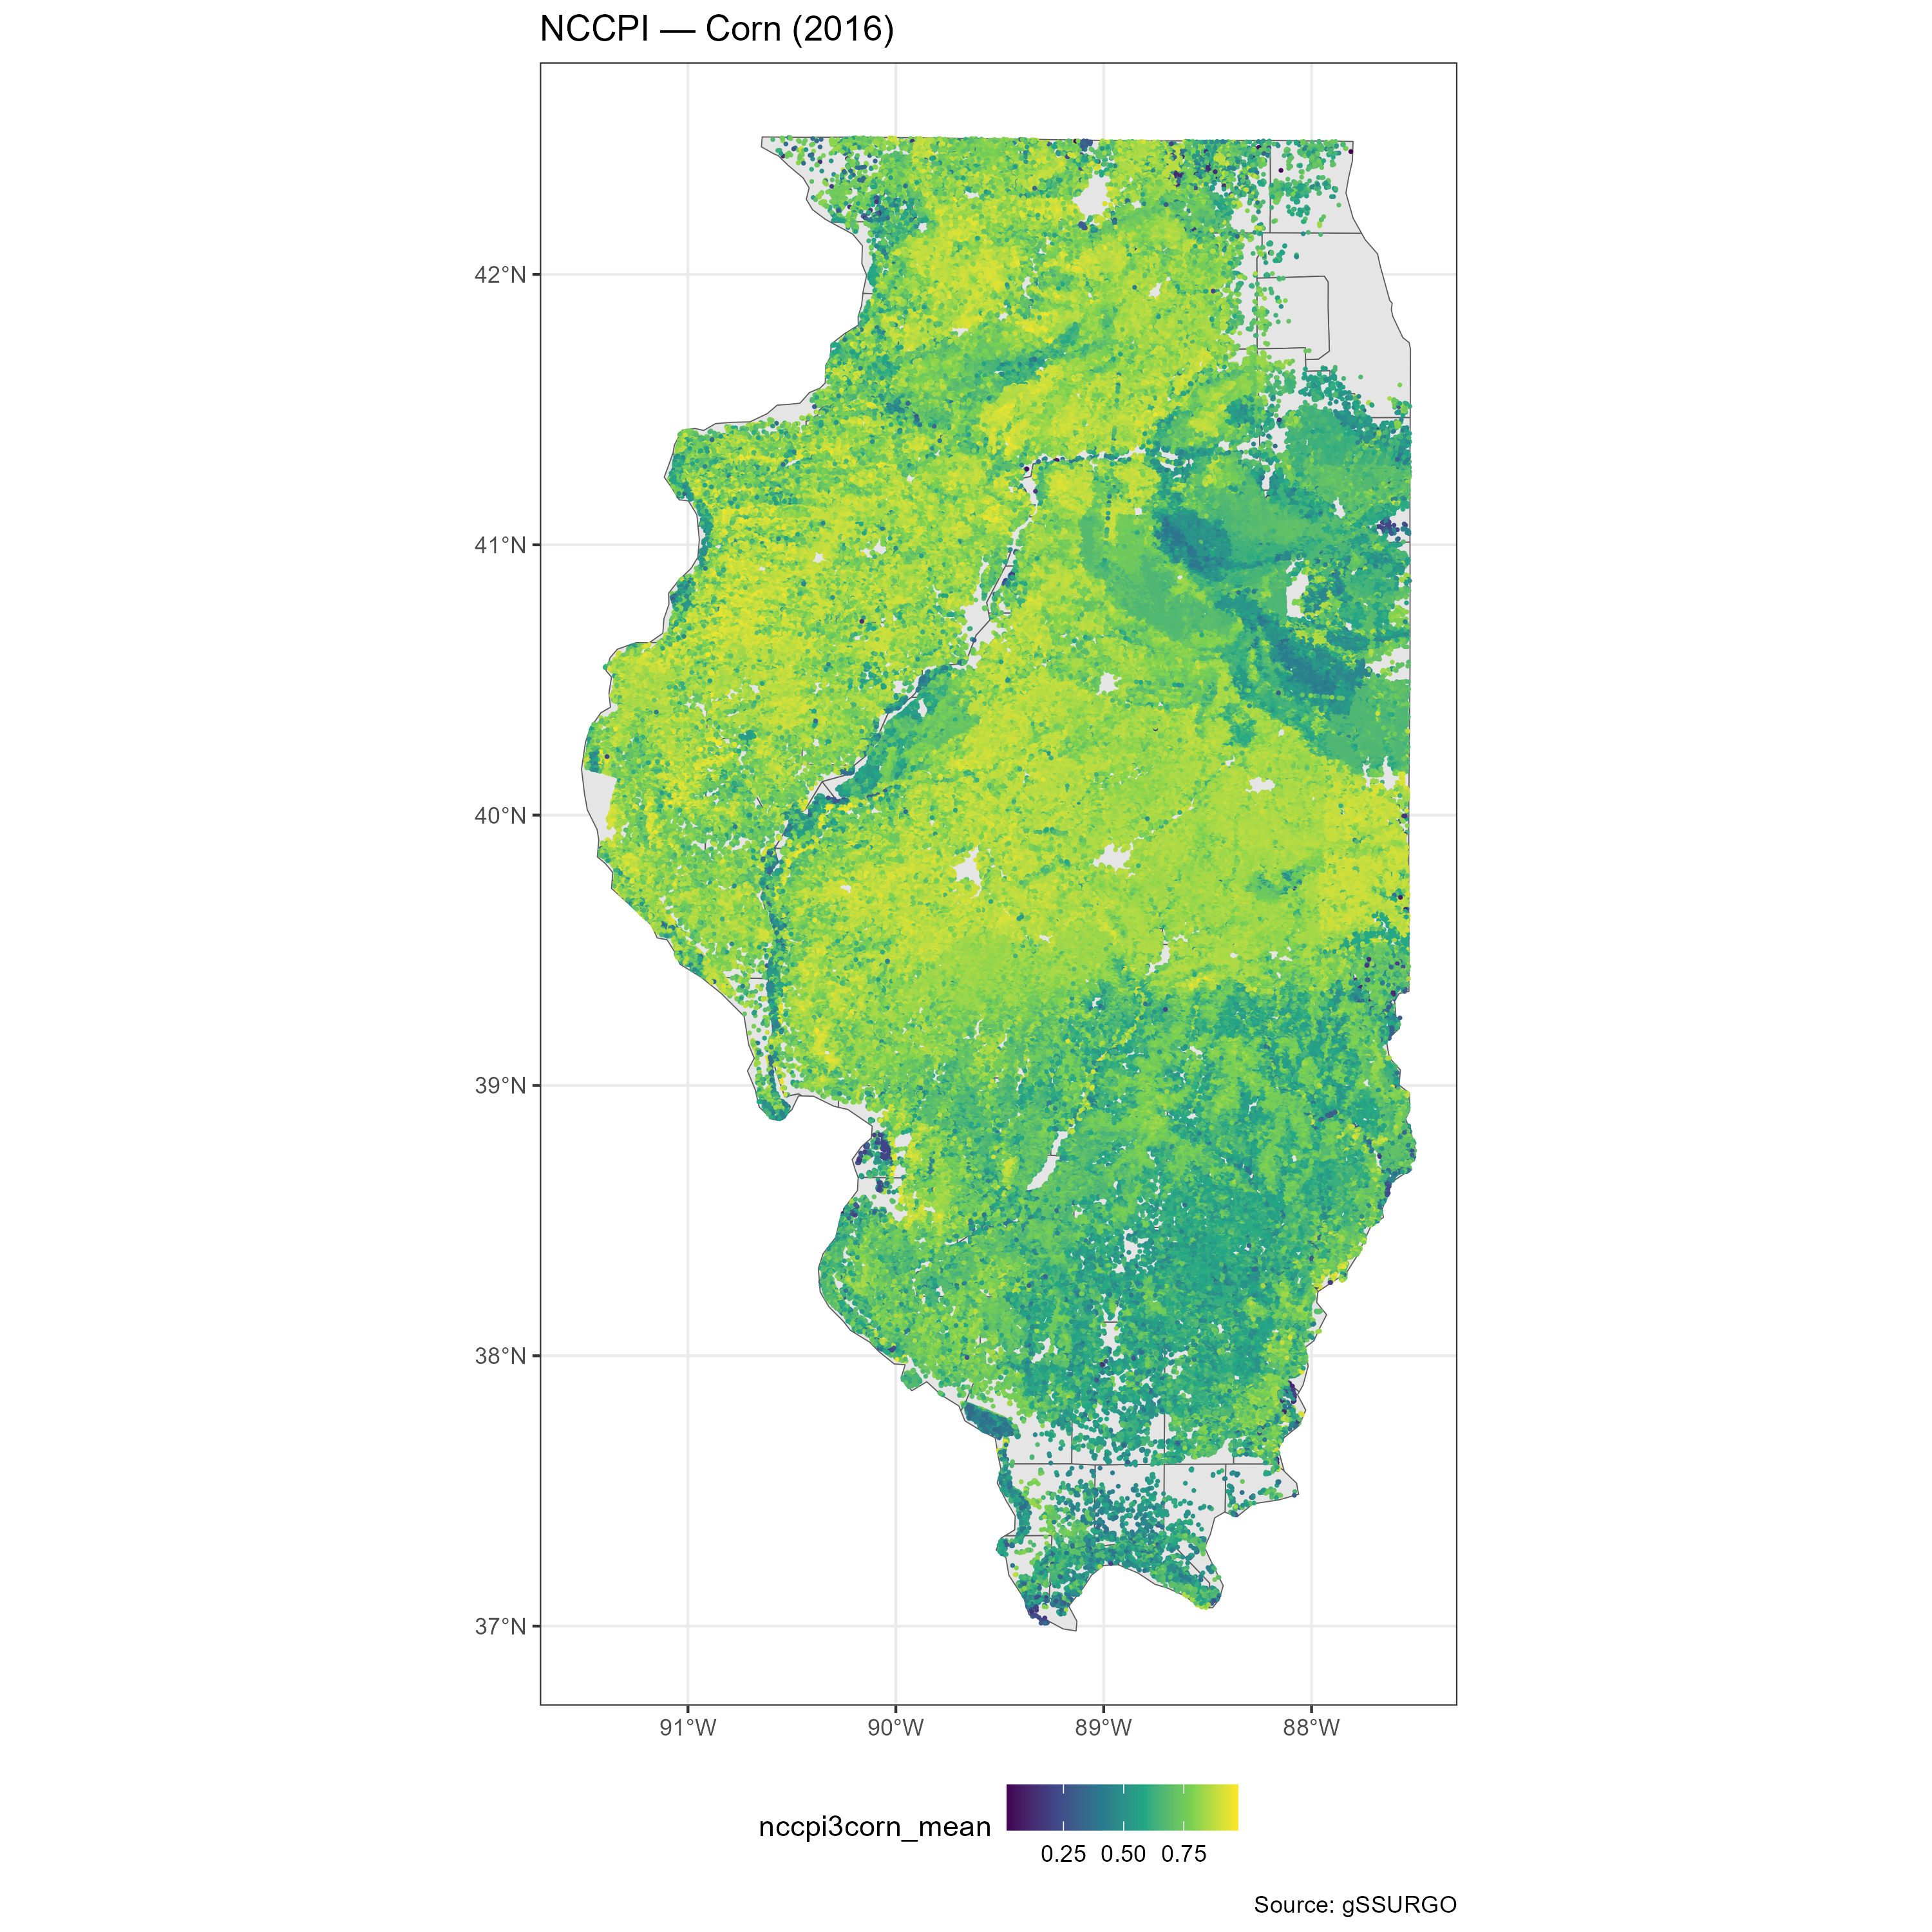
\includegraphics[width=0.85\textwidth]{figures/nccpi_corn_map}
  \caption{National Commodity Crop Productivity Index (corn) across Illinois.}
  \label{fig:nccpi_corn_map}
  \floatfoot{\footnotesize Notes: NCCPI corn values at 30-meter resolution.
  Source: gSSURGO, USDA-NRCS.}
\end{figure}

\end{document}
